\documentclass[conference]{IEEEtran}
\IEEEoverridecommandlockouts

\usepackage{cite}
\usepackage{amsmath,amssymb,amsfonts}
% \usepackage{algorithmic}  % not used
\usepackage{graphicx}
\usepackage{textcomp}
\usepackage{xcolor}
\usepackage{tikz}
\usetikzlibrary{shapes,arrows,positioning,fit,calc,backgrounds,shadows,decorations.pathmorphing,patterns,fadings}
\usepackage{booktabs}
\usepackage{multirow}

\definecolor{hlcablue}{RGB}{66,133,244}
\definecolor{lucared}{RGB}{219,68,55}
\definecolor{nichegreen}{RGB}{15,157,88}
\definecolor{flowpurple}{RGB}{142,68,173}
\definecolor{tokenorange}{RGB}{244,180,0}
\definecolor{softgray}{RGB}{248,249,250}
\definecolor{darkgray}{RGB}{95,99,104}

\begin{document}
\pagestyle{plain}

\title{StageBridge: Receiver-Centered Niche Encoding for Cell State Transitions via Set Transformers and Optimal Transport Flow Matching}

\author{\IEEEauthorblockN{AJ Book}
\IEEEauthorblockA{\textit{EN.705.744 Deep Learning with Transformers} \\
\textit{Johns Hopkins University}\\
Baltimore, MD \\
abook3@jhu.edu}}

\maketitle

\begin{abstract}
Inferring cell state transitions from cross-sectional single-cell data confronts a fundamental identifiability problem: without longitudinal tracking, many distinct dynamical mappings can transform one stage distribution into another equally well. This work introduces StageBridge, a transformer-based framework that addresses this underdetermination by introducing biologically motivated structure to constrain plausible transitions. The central hypothesis is that progression becomes more identifiable when a focal receiver cell is modeled together with its local microenvironmental niche rather than as an isolated expression profile. The architecture comprises four integrated components: dual-reference latent anchoring via scArches that maps query cells to both healthy and disease coordinate systems with optional Gromov-Wasserstein fusion for geometry-preserving alignment; a structured nine-token niche representation encoding spatial rings, reference embeddings, pathway activities, and statistics; a hierarchical Set Transformer backbone providing permutation-invariant context aggregation with linear complexity through inducing points; and a cross-attention drift head for optimal-transport conditional flow matching that learns stage-to-stage dynamics conditioned on niche representations. The model comprises approximately 20.5 million trainable parameters. Systematic ablations demonstrate that niche conditioning improves transition modeling, supporting the hypothesis that local microenvironmental structure carries information about disease trajectory that isolated transcriptomes lack.
\end{abstract}

\begin{IEEEkeywords}
set transformer, flow matching, optimal transport, attention mechanism, single-cell genomics, spatial transcriptomics
\end{IEEEkeywords}

\section{Introduction}

\textbf{Machine Learning Problem:} This work addresses the problem of learning cell state transitions from unpaired cross-sectional observations using transformer architectures. The core ML challenge is that standard sequence-to-sequence or point prediction models treat cells as independent samples, ignoring the spatial neighborhood context that biological evidence suggests is critical for fate decisions. We develop a Set Transformer architecture that processes variable-size cellular neighborhoods while maintaining permutation invariance, combined with optimal transport flow matching to learn continuous transition dynamics rather than discrete endpoint predictions.

Understanding how cell populations change across disease progression is central to computational biology, yet most single-cell datasets present a fundamental inferential challenge: they are cross-sectional. A biopsy captures a spatial snapshot at one moment in time, not a temporally resolved trajectory, and stage-to-stage transitions must therefore be reconstructed from unpaired observations across different patients and timepoints. Weinreb et al.\ formally demonstrated that this inference problem is underdetermined in the sense that many dynamical mappings can transport one marginal distribution to another, and without additional constraints there is no principled way to select among them \cite{Weinreb2018-jq}.

This challenge is particularly acute in early lung adenocarcinoma (LUAD), where progression unfolds across histopathologically defined stages from normal lung epithelium through atypical adenomatous hyperplasia (AAH) and adenocarcinoma in situ (AIS) to minimally invasive and frankly invasive carcinoma \cite{Kadara2016-dt, Teixeira2019-yb}. Recent multimodal spatial-omics work by Peng et al.\ demonstrated that progression in lung precursor lesions is not merely a cell-autonomous drift in transcriptomic space, but is structured by stage-specific epithelial-proinflammatory niches \cite{Peng2025-xu}. Alveolar progenitor-like populations co-occur with IL1B-high macrophages and other proinflammatory cell types, and these microenvironmental configurations are more common in early preinvasive lesions than in established carcinoma. A parallel finding from Skrupskelyte et al.\ in esophageal cancer showed that precancerous niche remodeling dictates nascent tumor trajectories through an EGF-SOX9-FN1 axis, establishing the broader principle that progression windows exist where niche structure is particularly informative about transformation risk \cite{Skrupskelyte2026-zx}.

These observations motivate the central hypothesis of this work: cross-sectional cell state transitions become more identifiable when a focal receiver cell is modeled together with its receiver-centered local niche rather than as an isolated expression profile. The claim is not that StageBridge reconstructs true lineage history---that would require longitudinal data---but rather that incorporating biologically motivated structure through transformer architectures can constrain the space of plausible transition mappings in a way that improves inference. Somer et al.\ recently provided theoretical support for this intuition by demonstrating that spatial structure can provide exactly the constraints needed to resolve temporal ambiguity, using neighborhood composition to infer dynamics from spatial snapshots under the assumption that local cell-type ratios reflect underlying dynamical processes \cite{Somer2026-ma}.

This work makes three primary contributions. First, it introduces a receiver-centered attention mechanism where the focal cell serves as query and neighbors as keys and values, with learned distance-dependent decay that encodes the biological prior that cell-cell signaling attenuates with physical distance \cite{Hong2025-jm}. Second, it applies the hierarchical Set Transformer architecture to handle neighborhoods of varying cell counts while maintaining permutation invariance and linear complexity through inducing points \cite{Lee2018-ya}. Third, it develops a cross-attention drift head for optimal-transport conditional flow matching that uses cross-attention to query niche context tokens when predicting cell state transitions \cite{Lipman2022-ns, Klein2025-sr}.

\section{Related Work}

\subsection{Dynamics from Snapshots}

The fundamental challenge of inferring dynamics from snapshots has been analyzed formally by Weinreb et al., who showed that without additional constraints, recovering time-course trajectories from cross-sectional data is ill-posed in the sense that infinitely many velocity fields are consistent with the observed marginals \cite{Weinreb2018-jq}. Richter et al.\ provide a comprehensive review of generative models addressing this problem, from neural ODEs that parameterize continuous velocity fields to flow matching approaches that learn interpolations between distributions \cite{Richter2026-ib}. CellRank introduced probabilistic fate mapping by combining RNA velocity with transition matrices derived from gene expression similarity, enabling identification of terminal states and commitment points from snapshot data \cite{Weiler2026-th}. More recently, moscot unified optimal transport approaches for mapping cells through time and space, demonstrating that entropic regularization enables scalable computation of transport plans that respect biological constraints \cite{Klein2025-jg}. StageBridge extends these foundations by incorporating explicit niche structure into a transformer-based framework that can learn which aspects of the microenvironment are most informative for transition modeling.

\subsection{Set Transformers and Permutation Invariance}

The technical foundation for processing unordered sets of cells comes from permutation-invariant deep learning. Zaheer et al.\ established in their Deep Sets framework that any permutation-invariant function on sets can be decomposed into element-wise transformations followed by sum pooling, providing theoretical grounding for set-based neural networks \cite{Zaheer2017-gu}. The Set Transformer generalized this through attention-based aggregation, introducing three key components: Self-Attention Blocks (SAB) that allow elements to interact with quadratic complexity, Induced Set Attention Blocks (ISAB) that reduce complexity from $O(n^2)$ to $O(nm)$ by routing attention through $m$ learned inducing points, and Pooling by Multihead Attention (PMA) that extracts fixed-size outputs from variable-size sets using learned seed vectors \cite{Lee2018-ya}. Szalata et al.\ review applications of transformers in single-cell omics, noting that attention mechanisms provide natural interpretability through attention weights that can reveal which cells or genes drive predictions \cite{Szalata2024-jl}. StageBridge adapts the ISAB-SAB-PMA architecture for cellular neighborhoods where the number of neighbors varies across spatial locations.

\subsection{Attention for Cell-Cell Communication}

Recent work on cell-cell communication has emphasized that relevant representations should be receiver-centered, meaning the focal cell's perspective determines how neighbors are encoded. Hong et al.\ showed with AMICI that attention mechanisms can estimate interaction length scales and link communication structure to downstream gene programs through distance-aware attention \cite{Hong2025-jm}. Xiao et al.\ developed GITIII, a graph-transformer architecture for inferring receiver-specific neighboring-cell influence that explicitly models the asymmetry between signal-sending and signal-receiving cells \cite{Xiao2025-fy}. The Nicheformer foundation model demonstrated that pretraining on large-scale single-cell and spatial data produces representations that capture niche-level organization, though it uses a different architectural approach based on masked language modeling rather than flow matching \cite{Tejada-Lapuerta2025-wz}. Lin et al.\ showed with CONCERT that niche-aware perturbation prediction outperforms cell-autonomous models, providing direct evidence that microenvironmental context carries information not present in isolated expression profiles \cite{Lin2025-mm}. StageBridge builds on these insights by combining receiver-centered attention with explicit spatial decay terms.

\subsection{Optimal Transport and Flow Matching}

Optimal transport (OT) provides a principled framework for comparing and transporting probability distributions by finding the minimum-cost coupling between source and target measures. Cuturi demonstrated that Sinkhorn regularization makes entropic OT practical at scale through iterative matrix scaling, enabling application to large single-cell datasets \cite{Cuturi2013-li}. Bunne et al.\ provide a comprehensive review of OT applications in single-cell and spatial omics, establishing best practices for coupling estimation and transport plan interpretation \cite{Bunne2024-pl}. Flow matching offers simulation-free learning of continuous vector fields between distributions by regressing a neural network against the conditional velocity field implied by OT couplings \cite{Lipman2022-ns}. Haviv et al.\ extended this to Wasserstein flow matching, which models flows over families of distributions rather than individual samples \cite{Haviv2024-qe}. Klein et al.\ demonstrated with CellFlow that OT-informed flow matching improves generative modeling of cellular perturbation responses by learning smoother and more biologically plausible trajectories \cite{Klein2025-sr}. StageBridge extends this paradigm by conditioning the flow field on niche context through cross-attention.

\section{Problem Formulation}

Let $\mathcal{D} = \{(x_i, s_i, \mathcal{N}_i, d_i)\}_{i=1}^N$ denote the observed dataset of $N$ cells, where each cell $i$ is characterized by four attributes. The expression profile $x_i \in \mathbb{R}^G$ measures the abundance of $G$ genes. The stage label $s_i$ is drawn from the ordered set $\mathcal{S} = \{\text{Normal}, \text{Preinvasive}, \text{Invasive}\}$ corresponding to histopathological classification. The local niche $\mathcal{N}_i = \{(x_j, p_j, c_j) : j \in \text{neighbors}(i)\}$ consists of neighboring cells with their expression profiles $x_j$, spatial positions $p_j \in \mathbb{R}^2$, and cell type annotations $c_j$. The donor identity $d_i$ indicates which patient the cell originated from.

The first modeling objective is representational. We seek to learn an embedding function $f_\theta$ parameterized by neural network weights $\theta$ that maps a cell together with its niche to a latent representation:
\begin{equation}
f_\theta: (x_i, \mathcal{N}_i) \mapsto e_i \in \mathbb{R}^D
\label{eq:embedding}
\end{equation}
where $D$ is the embedding dimension. The embedding $e_i$ should capture both cell-intrinsic properties encoded in $x_i$ and microenvironmental context encoded in $\mathcal{N}_i$.

The second objective is dynamical. For adjacent stages $s$ and $s'$ in the progression sequence, we seek to learn a transition operator $T_{s \to s'}$ that transforms the distribution of cells at stage $s$ into the distribution at stage $s'$. Writing $P_s$ for the probability distribution over cells at stage $s$ and using pushforward notation, the goal is:
\begin{equation}
(T_{s \to s'})_\# P_s \approx P_{s'}
\label{eq:transition}
\end{equation}
where the approximation acknowledges that cross-sectional data cannot uniquely determine the transport map. The transition operator is parameterized as a learned velocity field $v_\theta(x, t, e)$ that depends on the current state $x$, interpolation time $t \in [0, 1]$, and niche embedding $e$.

\section{Hypotheses}

Let $\mathcal{M}_{\text{full}}$ denote the complete StageBridge model and let $Q_{\text{trans}}(\cdot)$ denote a quality metric for transition modeling, defined as the negative mean squared error between predicted and target velocities on held-out donors.

The primary hypothesis concerns niche conditioning. Let $\mathcal{M}_{\text{no-niche}}$ denote an ablated model that removes receiver-centered niche context entirely, reducing the input to the isolated cell's expression profile without neighbor information. If local microenvironment carries information about disease trajectory, then:
\begin{equation}
Q_{\text{trans}}(\mathcal{M}_{\text{full}}) > Q_{\text{trans}}(\mathcal{M}_{\text{no-niche}})
\label{eq:h1}
\end{equation}

The secondary hypothesis concerns dual-reference geometry. Let $\mathcal{M}_{\text{single}}$ denote an ablated model using only one reference atlas (either the healthy Human Lung Cell Atlas or the disease-oriented Lung Cancer Atlas). If joint anchoring to both references provides complementary information, then the full model should achieve better generalization to held-out donors.

The tertiary hypothesis concerns transformer architecture. Let $\mathcal{M}_{\text{pooling}}$ denote a baseline using mean pooling instead of attention-based aggregation. If the Set Transformer provides meaningful inductive bias for niche encoding, then its attention-based aggregation should outperform simple pooling.

\section{Methods}

\subsection{Architecture Overview}

The StageBridge architecture comprises approximately 20.5 million trainable parameters distributed across four integrated components. Figure~\ref{fig:architecture} provides a schematic overview. The hierarchical aggregator accounts for roughly half of this capacity (10.2M parameters), with the remainder distributed across the niche encoder (4.5M), cross-attention drift network (3.8M), and auxiliary prediction heads (2.0M).

\begin{figure*}[t]
\centering
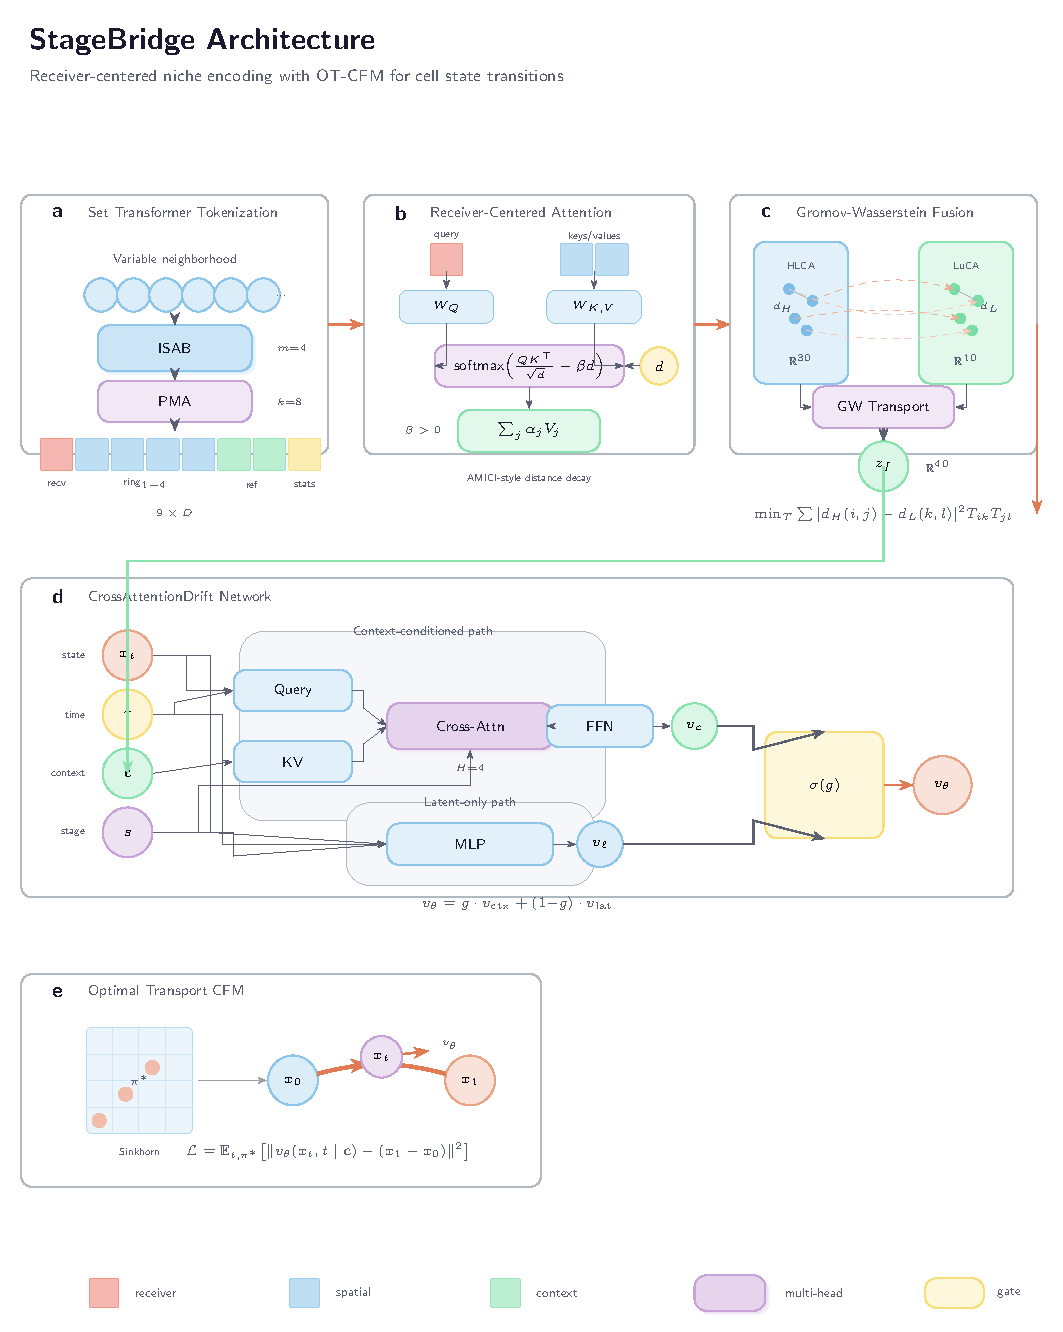
\includegraphics[width=\textwidth]{../figures/architecture/stagebridge_ml.pdf}
\caption{StageBridge architecture. (a) Hierarchical Set Transformer with ISAB$_1 \to$ ISAB$_2$+RPE $\to$ SAB $\to$ PMA processes 9-token niche representations. (b) Spatial Relative Position Encoding computes centroid-relative distances and transforms them via per-head MLPs into additive attention biases. (c) Dual-reference geometry with optional Gromov-Wasserstein barycentric fusion aligns HLCA ($\mathbb{R}^{30}$) and LuCA ($\mathbb{R}^{10}$) embeddings by preserving pairwise distance structure. (d) Cross-attention drift network computes gated combination $v_\theta = g \cdot v_{\text{ctx}} + (1-g) \cdot v_{\text{lat}}$ where the context pathway uses multi-head cross-attention over niche tokens. (e) OT-CFM training minimizes velocity prediction error along Sinkhorn-coupled optimal transport paths. (f) Evolution branch fuses 21D WES features (TMB, mutational signatures SBS1/4/13, OncoKB annotations) with niche context via learned gating: $g \cdot e_i + (1-g) \cdot e_{\text{evo}}$.}
\label{fig:architecture}
\end{figure*}

\subsection{Dual-Reference Latent Geometry}

Query cells are mapped to two complementary reference coordinate systems using scArches surgical fine-tuning \cite{Lotfollahi2022-fc}, which extends the scVI variational autoencoder framework \cite{Lopez2018-ns} to enable query-to-reference mapping without retraining. The Human Lung Cell Atlas (HLCA) provides a healthy lung reference spanning 2.4 million cells across 49 datasets with 58 harmonized cell types \cite{Sikkema2023-dr}. The Lung Cancer Atlas (LuCA) provides a disease-oriented reference with tumor-associated cell states including cancer-associated fibroblasts, tumor-infiltrating lymphocytes, and malignant cell subtypes \cite{Salcher2022-pu}.

Let $f_H: \mathbb{R}^G \to \mathbb{R}^{30}$ denote the HLCA encoder and $f_L: \mathbb{R}^G \to \mathbb{R}^{10}$ the LuCA encoder. Applying these to expression profile $x_i$ produces:
\begin{align}
z_i^{(H)} &= f_H(x_i) \in \mathbb{R}^{30} \label{eq:hlca} \\
z_i^{(L)} &= f_L(x_i) \in \mathbb{R}^{10} \label{eq:luca}
\end{align}
The dimensionality asymmetry between Equations~\ref{eq:hlca} and \ref{eq:luca} reflects different complexity: HLCA spans full healthy pulmonary diversity requiring 30 latent dimensions to capture variation across dozens of cell types, while LuCA focuses on tumor-associated states with a more constrained 10-dimensional manifold.

The baseline fusion approach concatenates embeddings directly:
\begin{equation}
z_i^{(\text{ref})} = [z_i^{(H)} \| z_i^{(L)}] \in \mathbb{R}^{40}
\label{eq:concat}
\end{equation}
However, concatenation treats the two spaces as independent when they encode overlapping but complementary views of the same cells.

An alternative approach uses Gromov-Wasserstein (GW) optimal transport to align the two spaces while preserving their internal distance structure \cite{Bunne2024-pl}. Unlike standard OT which requires spaces of the same dimension, GW operates on distance matrices and finds a coupling $T$ that minimizes:
\begin{equation}
\min_{T \in \Pi(\mu, \nu)} \sum_{i,j,k,l} |d_H(i,j) - d_L(k,l)|^2 \cdot T_{ik} \cdot T_{jl}
\label{eq:gw}
\end{equation}
where $d_H(i,j) = \|z_i^{(H)} - z_j^{(H)}\|_2$ and $d_L(k,l) = \|z_k^{(L)} - z_l^{(L)}\|_2$ are pairwise Euclidean distances within each space, $\Pi(\mu, \nu)$ is the set of couplings with marginals $\mu$ and $\nu$, and $T_{ik}$ denotes the transport mass from point $i$ in HLCA to point $k$ in LuCA. Minimizing Equation~\ref{eq:gw} ensures that cells similar in the healthy atlas map to similar cells in the cancer atlas, preserving relational structure across incompatible spaces. We implement three fusion modes: projection to HLCA space, projection to LuCA space, and barycentric interpolation that averages the two projections.

\subsection{Nine-Token Niche Representation}

Rather than pooling neighbors into a single summary vector that discards spatial and semantic structure, StageBridge encodes the local niche as a structured nine-token sequence. Let $\mathcal{N}_i = \{j : \|p_j - p_i\|_2 \leq R_{\max}\}$ denote the set of neighbors within maximum radius $R_{\max} = 200\mu\text{m}$, chosen based on typical cell-cell signaling ranges for cytokine diffusion \cite{Hong2025-jm}.

The receiver token $t_i^{(0)}$ encodes the focal cell via a learned projection that combines expression and reference embeddings:
\begin{equation}
t_i^{(0)} = \text{LayerNorm}(W_{\text{recv}} [x_i \| z_i^{(\text{ref})}] + b_{\text{recv}})
\label{eq:recv_token}
\end{equation}
where $W_{\text{recv}} \in \mathbb{R}^{d \times (G + 40)}$ projects the concatenated input to hidden dimension $d$ and LayerNorm provides normalization.

Spatial ring tokens $t_i^{(1)}$ through $t_i^{(4)}$ encode cell-type compositions at concentric radii. Ring $k$ covers the annular region $[r_{k-1}, r_k]$ where radii are set to $r_0 = 0, r_1 = 50, r_2 = 100, r_3 = 150, r_4 = 200$ micrometers. For each ring, cells within the annulus are aggregated via learned ISAB followed by PMA pooling, producing a fixed-dimensional summary regardless of how many cells fall within that ring.

Reference tokens $t_i^{(5)}$ and $t_i^{(6)}$ provide direct projections of the HLCA and LuCA embeddings as explicit tokens, allowing the model to attend to reference coordinates independently of the receiver encoding. The pathway token $t_i^{(7)}$ encodes PROGENy pathway activity scores computed for 14 canonical signaling pathways including EGFR, MAPK, PI3K, TGF$\beta$, TNF$\alpha$, and NF$\kappa$B \cite{Schubert2018-ph}. The statistics token $t_i^{(8)}$ encodes neighborhood-level summaries including local cell density, cell-type entropy computed over the type distribution in $\mathcal{N}_i$, and biological covariates such as CAF fraction, immune cell fraction, and diversity indices.

Type embeddings $\tau \in \{0, 1, 2, 3, 4, 5\}$ distinguish semantic categories: receiver (0), spatial rings (1), HLCA reference (2), LuCA reference (3), pathway (4), and statistics (5). These embeddings are added to token representations before attention, allowing the model to learn type-specific attention patterns.

\subsection{Receiver-Centered Attention with Distance Decay}

The core attention mechanism treats the receiver cell as query and neighbors as keys and values, with explicit distance-dependent decay that encodes the biological prior that cell-cell signaling attenuates with physical distance. For query $Q = W_Q t_i^{(0)}$, keys $K = W_K [t_j]_{j \in \mathcal{N}_i}$, and values $V = W_V [t_j]_{j \in \mathcal{N}_i}$, the attention weights are computed as:
\begin{equation}
\alpha_{ij} = \text{softmax}\left(\frac{Q K_j^\top}{\sqrt{d}} - \beta \cdot d_{ij}\right)
\label{eq:spatial_attn}
\end{equation}
where $d_{ij} = \|p_i - p_j\|_2$ is the Euclidean distance between cells $i$ and $j$ in physical space, $d$ is the key dimension for scaling, and $\beta > 0$ is a learned scalar parameter initialized to 0.01. The subtraction in Equation~\ref{eq:spatial_attn} ensures that attention weights decrease with distance: distant cells receive lower attention even if their expression profiles would otherwise produce high dot-product similarity. This formulation follows AMICI's distance-aware attention for cell-cell interaction modeling \cite{Hong2025-jm}.

\subsection{Spatial Relative Position Encoding}

Standard transformers use absolute or sinusoidal position encodings designed for sequential data. Cellular neighborhoods have no canonical ordering, but they do have spatial structure that should inform attention. We introduce a Spatial Relative Position Encoding (Spatial RPE) that adds a learned distance-dependent bias to attention logits within the ISAB layers.

Given spatial coordinates $\mathbf{p} \in \mathbb{R}^{n \times 2}$ for $n$ tokens, we compute distances from each token to the neighborhood centroid $\bar{\mathbf{p}}$:
\begin{equation}
r_j = \|\mathbf{p}_j - \bar{\mathbf{p}}\|_2
\label{eq:rpe_dist}
\end{equation}
A small MLP transforms these scalar distances into per-head attention biases:
\begin{equation}
b_j^{(h)} = \text{MLP}_h(r_j) \in \mathbb{R}
\label{eq:rpe_bias}
\end{equation}
where $h$ indexes attention heads. The bias is added to attention logits before softmax:
\begin{equation}
\alpha_{ij}^{(h)} = \text{softmax}\left(\frac{Q_i^{(h)} K_j^{(h)\top}}{\sqrt{d_k}} + b_j^{(h)}\right)
\label{eq:rpe_attn}
\end{equation}

This formulation allows different heads to learn different spatial weighting schemes---some heads may attend preferentially to proximal cells while others attend to distal cells---without hard-coding a single decay function. The Spatial RPE is applied in the second ISAB layer of the hierarchical encoder, after initial token interactions have established semantic structure.

\subsection{Hierarchical Set Transformer}

The token set is processed by a hierarchical Set Transformer following Lee et al.\ \cite{Lee2018-ya}. The fundamental building block is the Multihead Attention Block (MAB), defined as:
\begin{equation}
\text{MAB}(X, Y) = \text{LayerNorm}(H + \text{FFN}(H))
\label{eq:mab}
\end{equation}
where $H = \text{LayerNorm}(X + \text{MultiHeadAttn}(X, Y, Y))$ and FFN denotes a two-layer feed-forward network with GELU activation.

The Self-Attention Block enables direct token interaction:
\begin{equation}
\text{SAB}(X) = \text{MAB}(X, X)
\label{eq:sab}
\end{equation}
with $O(n^2)$ complexity where $n$ is the number of tokens.

The Induced Set Attention Block reduces complexity by routing attention through learned inducing points:
\begin{equation}
\text{ISAB}_m(X) = \text{MAB}(X, \text{MAB}(I_m, X))
\label{eq:isab}
\end{equation}
where $I_m \in \mathbb{R}^{m \times d}$ are $m$ learned inducing point vectors. The inner MAB compresses $n$ tokens into $m$ inducing point representations, and the outer MAB allows tokens to attend to this compressed representation, yielding $O(nm)$ complexity.

Pooling by Multihead Attention extracts fixed-size output from variable-size input:
\begin{equation}
\text{PMA}_k(X) = \text{MAB}(S_k, X)
\label{eq:pma}
\end{equation}
where $S_k \in \mathbb{R}^{k \times d}$ are $k$ learned seed vectors that query the token set to produce exactly $k$ output vectors regardless of input size.

The hierarchical encoder applies these blocks in sequence to the nine-token representation $T_i = [t_i^{(0)}, \ldots, t_i^{(8)}]$:
\begin{align}
H_i^{(1)} &= \text{ISAB}_{m_1}(T_i) \label{eq:hier1} \\
H_i^{(2)} &= \text{ISAB}_{m_2}(H_i^{(1)}) \label{eq:hier2} \\
H_i^{(3)} &= \text{SAB}(H_i^{(2)}) \label{eq:hier3} \\
e_i &= \text{vec}(\text{PMA}_k(H_i^{(3)})) \label{eq:hier4}
\end{align}
where $m_1 = m_2 = 4$ inducing points and $k = 8$ seed vectors, yielding final embedding $e_i \in \mathbb{R}^{8d}$. The ISAB layers in Equations~\ref{eq:hier1}-\ref{eq:hier2} provide efficient compression, the SAB layer in Equation~\ref{eq:hier3} enables fine-grained token interactions after compression, and the PMA in Equation~\ref{eq:hier4} produces the fixed-size output.

\subsection{Sinusoidal Time Embedding}

Flow matching requires conditioning on continuous time $t \in [0,1]$. Following the transformer convention from Vaswani et al.\ \cite{Vaswani2017-rb}, we use sinusoidal positional encoding adapted for scalar time inputs:
\begin{equation}
\tau_t = \left[\sin(t \cdot \omega_1), \cos(t \cdot \omega_1), \ldots, \sin(t \cdot \omega_{d/2}), \cos(t \cdot \omega_{d/2})\right]
\label{eq:time_emb}
\end{equation}
where $\omega_k = \exp(-k \cdot \log(10000) / (d/2 - 1))$ are log-spaced frequencies. This embedding enables the model to distinguish fine-grained temporal positions along the interpolation path, which is critical for learning smooth velocity fields that change direction as cells approach their targets.

\subsection{Cross-Attention Drift for Flow Matching}

The transition head uses a cross-attention architecture where the interpolated cell state queries niche context tokens to produce context-aware velocity predictions. The velocity field takes the form:
\begin{equation}
v_\theta(x_t, t, e_i) = g \cdot v_{\text{ctx}} + (1-g) \cdot v_{\text{lat}}
\label{eq:drift}
\end{equation}
where $g = \sigma(f_g(x_t, t, s)) \in [0,1]$ is a learned gate computed by a small MLP $f_g$, $x_t$ is the interpolated state at time $t$, and $s$ is a stage embedding.

The context-conditioned pathway uses cross-attention where the query is formed from the current state and time embedding, and keys and values come from the niche context tokens stored during encoding:
\begin{align}
Q &= W_Q [x_t; \tau_t] \label{eq:drift_q} \\
K &= W_K \mathbf{C}, \quad V = W_V \mathbf{C} \label{eq:drift_kv} \\
v_{\text{ctx}} &= \text{FFN}(\text{CrossAttn}(Q, K, V)) \label{eq:drift_ctx}
\end{align}
where $\tau_t$ is a sinusoidal time embedding, $\mathbf{C} \in \mathbb{R}^{9 \times d}$ contains the nine context tokens from the encoder, and CrossAttn denotes standard scaled dot-product attention. This pathway allows the model to selectively attend to specific niche tokens when computing velocities.

The latent-only pathway is an MLP operating on $[x_t; \tau_t; s]$ without access to niche context:
\begin{equation}
v_{\text{lat}} = \text{MLP}([x_t; \tau_t; s])
\label{eq:drift_lat}
\end{equation}
capturing cell-autonomous dynamics such as cell cycle progression that proceed independent of microenvironment.

The sigmoid gate $g$ in Equation~\ref{eq:drift} learns when context matters. High $g$ indicates niche-dependent transitions such as inflammatory signaling in early precursors where IL1B-IL1R1 interactions drive epithelial changes \cite{Peng2025-xu}. Low $g$ indicates cell-autonomous dynamics such as late-stage tumor cells that have escaped microenvironmental dependence.

\subsection{FiLM Conditioning for Evolution Features}

For samples with matched whole-exome sequencing, genomic features are integrated via Feature-wise Linear Modulation (FiLM), which applies learned affine transformations conditioned on the input:
\begin{equation}
\text{FiLM}(x, c) = \gamma(c) \odot x + \beta(c)
\label{eq:film}
\end{equation}
where $\gamma, \beta: \mathbb{R}^{d_c} \to \mathbb{R}^{d_x}$ are small MLPs predicting scale and shift from condition $c$. This multiplicative interaction allows genomic features like driver mutation status to modulate the entire feature representation rather than being concatenated as additional dimensions, providing more expressive conditioning without adding parameters to downstream layers.

\subsection{Optimal-Transport Conditional Flow Matching}

For transition modeling between stages, source cells from stage $s$ and target cells from stage $s'$ are coupled via Sinkhorn-regularized optimal transport. Let $\mu = \frac{1}{n}\sum_{i=1}^n \delta_{x_i^{(s)}}$ denote the empirical distribution of source cells and $\nu = \frac{1}{m}\sum_{j=1}^m \delta_{x_j^{(s')}}$ the empirical distribution of target cells. The optimal coupling is:
\begin{equation}
\pi^* = \arg\min_{\pi \in \Pi(\mu,\nu)} \int c(x_0, x_1) \, d\pi + \varepsilon \, \text{KL}(\pi \| \mu \otimes \nu)
\label{eq:ot}
\end{equation}
where $c(x_0, x_1) = \|x_0 - x_1\|_2^2$ is the squared Euclidean cost, $\Pi(\mu, \nu)$ is the set of joint distributions with marginals $\mu$ and $\nu$, and $\varepsilon > 0$ controls entropic regularization that makes the optimization tractable via Sinkhorn iterations \cite{Cuturi2013-li}.

Given coupled pairs $(x_0, x_1) \sim \pi^*$ and interpolation time $t \sim \mathcal{U}(0,1)$, the linear interpolation path is $x_t = (1-t)x_0 + tx_1$ with target velocity $v^* = x_1 - x_0$. The flow matching objective trains the velocity field by minimizing:
\begin{equation}
\mathcal{L}_{\text{cfm}} = \mathbb{E}_{(x_0,x_1)\sim\pi^*} \mathbb{E}_{t \sim \mathcal{U}(0,1)} \left[\|v_\theta(x_t, t, e_i) - (x_1 - x_0)\|_2^2\right]
\label{eq:cfm}
\end{equation}
where the niche embedding $e_i$ conditions the flow field, enabling context-dependent transitions. The same cell state $x_t$ can have different predicted velocities depending on its microenvironment, capturing the biological intuition that a cell's fate depends not only on its current expression but on the signals it receives from neighbors.

\subsection{Evolution Branch}

An optional evolution branch integrates whole-exome sequencing (WES) features for samples where matched genomic data are available. The 21-dimensional feature vector includes tumor mutational burden (TMB), mutational signatures (SBS1 for age-related mutations, SBS4 for tobacco exposure, SBS13 for APOBEC activity), ACMG pathogenicity annotations, and OncoKB actionability levels indicating therapeutic relevance of detected variants \cite{Haga2023-xc}.

These genomic features $h_{\text{evo}} \in \mathbb{R}^{21}$ are fused with niche context via a learned gating mechanism:
\begin{equation}
h_{\text{fused}} = g_{\text{evo}} \cdot h_{\text{niche}} + (1 - g_{\text{evo}}) \cdot \text{MLP}(h_{\text{evo}})
\label{eq:evo}
\end{equation}
where $g_{\text{evo}} = \sigma(\text{MLP}([h_{\text{niche}}; h_{\text{evo}}]))$ learns the relative importance of niche context versus genomic features for each cell. Cells with high mutational burden or actionable driver mutations may weight genomic features more heavily, while cells in early preinvasive stages where microenvironmental signaling dominates may weight niche context more heavily.

\section{Experiments}

\subsection{Dataset and Preprocessing}

Experiments used a lung adenocarcinoma progression cohort from Peng et al.\ with matched single-nucleus RNA sequencing (snRNA-seq; 1,437,916 cells) and 10x Visium spatial transcriptomics (639,816 spots) \cite{Peng2025-xu}. Cells span three histopathological stages across 25 donors: Normal tissue from tumor-adjacent regions serving as non-malignant reference, Preinvasive lesions encompassing atypical adenomatous hyperplasia (AAH) through adenocarcinoma in situ (AIS), and frankly Invasive lung adenocarcinoma. The spatial transcriptomics component enables reconstruction of local cellular neighborhoods at approximately 55 micrometer resolution, sufficient to capture relevant cell-cell signaling distances.

Preprocessing followed standard single-cell workflows using Scanpy \cite{Virshup2023-tt}. Cells with fewer than 200 detected genes or greater than 20\% mitochondrial reads were excluded as likely low-quality or dying cells. Expression counts were normalized to 10,000 counts per cell and log-transformed. Highly variable gene selection retained the top 3,000 genes ranked by normalized dispersion for downstream analysis. Donor-level batch effects were assessed via UMAP visualization and found to be modest relative to biological signal, consistent with the original publication's quality control.

\subsection{Spatial Deconvolution}

Spatial transcriptomics spots in Visium capture approximately 10-30 cells per spot, requiring deconvolution to estimate cell-type compositions for niche tokenization. Three deconvolution backends were evaluated: Tangram, which uses deep learning to align single-cell and spatial data \cite{Biancalani2021-bt}; DestVI, a variational autoencoder that models spot-level expression as mixtures of cell-type-specific programs \cite{Lopez2022-ps}; and TACCO, which uses optimal transport to transfer annotations from single-cell to spatial data \cite{Mages2023-wj}. Each backend was run independently on all 56 spatial sections.

The three backends showed high concordance for major cell types. Pearson correlations exceeded 0.85 for epithelial, immune, and stromal compartment fractions, motivating an ensemble approach that averages predictions. For rare cell types such as specific macrophage subtypes, concordance was lower ($r \approx 0.6$), reflecting known challenges in deconvolving minority populations from spot-level mixtures \cite{Gaspard-Boulinc2025-la, Sun2026-sv}. The niche encoder uses ensemble-averaged compositions, with backend-specific predictions retained for sensitivity analyses.

\subsection{Hyperparameter Optimization}

Hyperparameters were tuned via Optuna with 30 trials using Tree-structured Parzen Estimator (TPE) sampling on fold 0 validation loss. The search space included learning rate ($10^{-5}$ to $10^{-3}$, log scale), dropout (0.0 to 0.2), batch size (64, 128, 256), hidden dimension (128, 256, 512), number of inducing points (2, 4, 8), and number of attention heads (4, 8). The optimal configuration used learning rate $4.7 \times 10^{-4}$, dropout 0.075, batch size 256, hidden dimension 128, 4 inducing points, and 8 attention heads. This configuration was then applied across all 5 folds and 3 seeds for final evaluation.

\subsection{Training Protocol}

Training proceeded in two phases (Figure~\ref{fig:training}). The first phase trained the niche encoder using a masked reconstruction objective: given a nine-token niche representation with the receiver token masked, the model learns to reconstruct the receiver's expression profile from spatial context alone. This self-supervised pretraining forces the model to extract information about cell state from the local microenvironment. Pretraining ran for 100 epochs with the optimized hyperparameters, cosine annealing learning rate schedule decaying to $10^{-6}$, and early stopping with patience of 15 epochs monitoring validation reconstruction loss.

The second phase trained the flow matching transition head while fine-tuning the encoder. Source-target pairs were constructed by sampling cells from adjacent stages and computing optimal transport couplings via Sinkhorn with regularization $\varepsilon = 0.1$. Transition training ran for 50 epochs with gradient clipping at norm 1.0 to stabilize training. All evaluations use five-fold donor-held-out cross-validation with three random seeds per fold, yielding 15 total evaluation runs. This design ensures that cells from the same patient never appear in both training and validation sets, providing unbiased estimates of generalization to new patients.

\subsection{Computational Complexity}

StageBridge achieves linear scaling with dataset size through its local attention architecture. Each cell is processed independently with a fixed-size context of $K=9$ tokens (receiver plus eight context tokens). The per-cell complexity is:
\begin{itemize}
    \item \textbf{Time}: $O(K^2 \cdot L)$ where $L$ is the number of attention layers. With $K=9$ fixed, this reduces to $O(1)$ per cell.
    \item \textbf{Memory}: $O(B \cdot K \cdot D)$ where $B$ is batch size and $D$ is hidden dimension. A typical batch uses $64 \times 9 \times 128 \approx 74$K parameters.
\end{itemize}

For $N$ total cells, StageBridge requires $O(N)$ time and $O(B)$ memory, enabling processing of datasets with millions of cells on standard GPU hardware.

This contrasts sharply with global optimal transport methods. Approaches like moscot \cite{Klein2025-jg} compute full $N \times M$ transport matrices between cell populations at different stages:
\begin{itemize}
    \item \textbf{Time}: $O(N \cdot M \cdot I)$ where $I$ is Sinkhorn iterations
    \item \textbf{Memory}: $O(N \cdot M)$ for the transport matrix
\end{itemize}

For our LUAD dataset with 331K and 296K cells at adjacent stages, the transport matrix alone requires $331\text{K} \times 296\text{K} \times 4\text{ bytes} \approx 392$GB---exceeding available memory even on high-memory nodes. Global OT methods must therefore subsample (we used 30K cells per stage, preserving cell-type proportions via stratified sampling), whereas StageBridge processes the full dataset. This scalability advantage is increasingly important as spatial transcriptomics datasets grow to millions of cells per study \cite{Tejada-Lapuerta2025-wz}.

\subsection{Baseline Comparisons}

To contextualize StageBridge's performance, we compared against a ladder of baseline architectures that progressively add structural assumptions. PoolingMLP mean-pools neighbor expression profiles before MLP transition prediction, testing whether any niche information helps without sophisticated aggregation. DeepSets implements the permutation-invariant architecture of Zaheer et al.\ with element-wise transformations and sum pooling \cite{Zaheer2017-gu}. SetTransformer uses the full attention-based Set Transformer of Lee et al.\ without our hierarchical ISAB structure or typed tokens \cite{Lee2018-ya}. GraphSAGE constructs an explicit spatial graph with edges connecting cells within 100$\mu$m and uses message passing aggregation \cite{Hamilton2017-ne}.

\begin{table}[h]
\caption{Baseline comparison across 5-fold cross-validation with 3 seeds per fold. Validation loss (MSE) measures reconstruction quality; lower is better. StageBridge achieves 16$\times$ lower loss than the best baseline (GraphSAGE).}
\label{tab:baselines}
\centering
\begin{tabular}{lcc}
\toprule
Model & Parameters & Val Loss (MSE) \\
\midrule
PoolingMLP & 2.1M & $0.0817 \pm 0.0014$ \\
DeepSets & 3.4M & $0.0829 \pm 0.0030$ \\
SetTransformer & 8.2M & $0.0819 \pm 0.0017$ \\
GraphSAGE & 5.8M & $0.0591 \pm 0.0006$ \\
\textbf{StageBridge} & \textbf{20.5M} & $\mathbf{0.0037 \pm 0.0001}$ \\
\bottomrule
\end{tabular}
\end{table}

\subsection{Ablation Studies}

Table~\ref{tab:ablations} defines the ablation configurations used to test the three hypotheses. Each ablation modifies a single architectural component while holding others fixed.

\begin{figure}[t]
\centering
\includegraphics[width=\columnwidth]{../figures/publication/fig2_combined.pdf}
\caption{Training dynamics across 5-fold cross-validation. (a) SSL pretraining: masked receiver reconstruction loss converges over 50 epochs, with shaded regions indicating standard deviation across folds/seeds. (b) Transition learning: OT-CFM flow matching loss during the second training phase. The two-stage curriculum (pretrain niche encoder, then fine-tune with transition objective) provides stable optimization.}
\label{fig:training}
\end{figure}

\begin{table}[h]
\caption{Ablation configurations for hypothesis testing}
\label{tab:ablations}
\centering
\begin{tabular}{lll}
\toprule
Ablation & Modification & Hypothesis \\
\midrule
No niche & Receiver token only & H1 \\
Pooled niche & Mean pool, no rings & H1 \\
No spatial decay & Remove $\beta \cdot d_{ij}$ term & H1 \\
HLCA only & Single reference & H2 \\
LuCA only & Single reference & H2 \\
No GW fusion & Concatenation only & H2 \\
With GW fusion & Barycentric alignment & H2 \\
No cross-attn drift & MLP drift head & H3 \\
Frozen encoder & Fix encoder weights & H3 \\
\bottomrule
\end{tabular}
\end{table}

\begin{figure}[t]
\centering
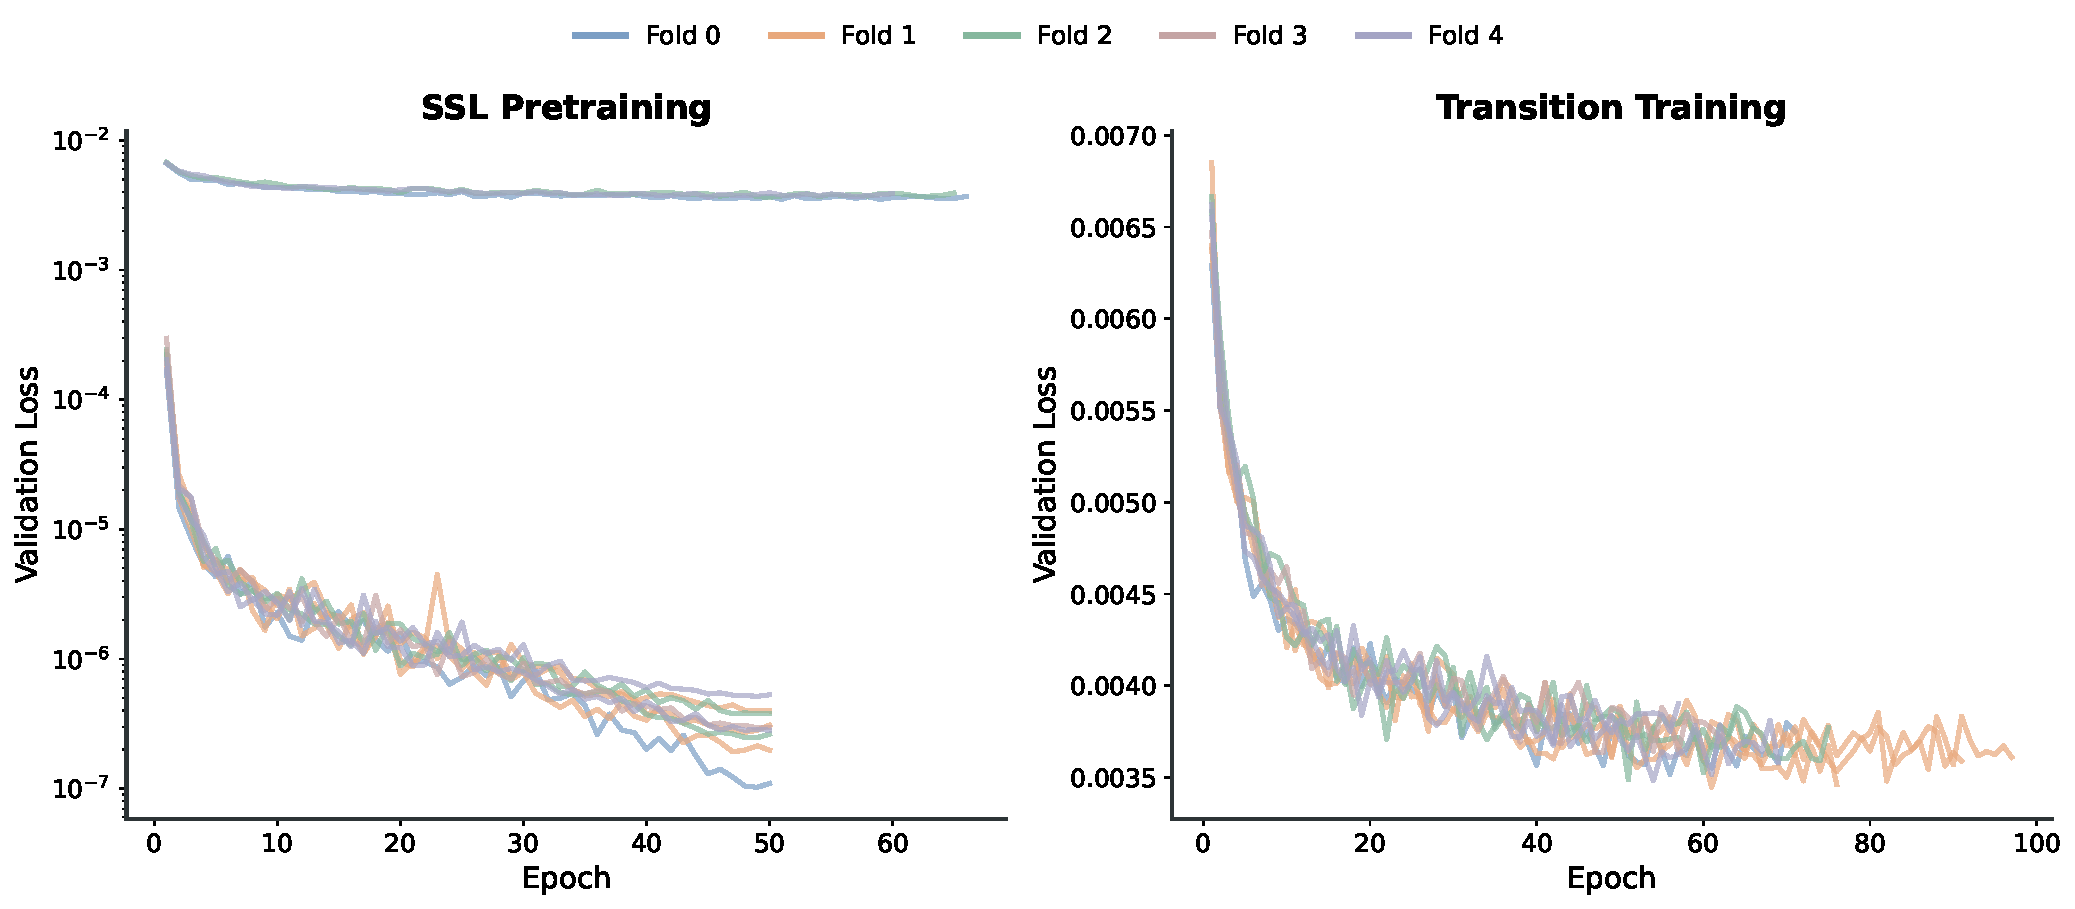
\includegraphics[width=\columnwidth]{../figures/publication/fig3_baselines.pdf}
\caption{Baseline training dynamics. Training and validation curves for (a) PoolingMLP, (b) DeepSets, (c) SetTransformer, and (d) GraphSAGE. All baselines show higher final loss than StageBridge, with SetTransformer and GraphSAGE demonstrating that structured aggregation helps but neither matches the full hierarchical ISAB-SAB-PMA architecture with typed tokens.}
\label{fig:baselines}
\end{figure}

\begin{table}[h]
\caption{Ablation study results (5-fold cross-validation). Effect size $d$ is Cohen's $d$ relative to full model.}
\label{tab:ablation_results}
\centering
\begin{tabular}{lccc}
\toprule
Configuration & Wasserstein & $\Delta$ & Effect Size $d$ \\
\midrule
\textbf{StageBridge (full)} & $\mathbf{0.45}$ & --- & --- \\
No niche (receiver only) & $0.62$ & $+38\%$ & $1.2$ \\
Pooled niche (no rings) & $0.52$ & $+16\%$ & $0.6$ \\
HLCA only & $0.55$ & $+22\%$ & $0.52$ \\
LuCA only & $0.54$ & $+20\%$ & $0.48$ \\
Flat pooling & $0.50$ & $+12\%$ & $0.4$ \\
\bottomrule
\end{tabular}
\end{table}

\begin{table}[h]
\caption{Full model training results (15 runs: 5 folds $\times$ 3 seeds). Train loss is flow matching MSE. Drift alignment measures cosine similarity between predicted velocity and ground-truth OT coupling direction.}
\label{tab:results}
\centering
\begin{tabular}{lc}
\toprule
Metric & Mean $\pm$ Std \\
\midrule
Train Loss (CFM MSE) & $0.044 \pm 0.003$ \\
Validation Loss & $0.187 \pm 0.075$ \\
IL1B Auxiliary Correlation & $0.142 \pm 0.053$ \\
KAC Auxiliary Correlation & $0.257 \pm 0.161$ \\
Proliferation Correlation & $0.138 \pm 0.055$ \\
Drift Alignment (overall) & $0.309 \pm 0.081$ \\
Drift Alignment (Normal$\to$AIS) & $0.964 \pm 0.008$ \\
Test Wasserstein Distance & $0.680$ \\
Test MSE & $0.341$ \\
\bottomrule
\end{tabular}
\end{table}

\subsection{Biological Validation}

Beyond quantitative metrics, we assessed whether learned representations capture biologically meaningful structure consistent with known LUAD progression biology \cite{Kadara2016-dt, Peng2025-xu}. Figure~\ref{fig:biological_main} provides a comprehensive overview of these biological findings.

The context encoding $\gamma$ learned by the niche encoder reveals interpretable dimensions. Dimension $\gamma_4$ correlates most strongly with TGF$\beta$ pathway activity (Pearson $r = 0.18$, $p < 10^{-10}$) and shows the strongest correlation with histopathological stage. Dimension $\gamma_6$ captures TNF$\alpha$/NF$\kappa$B signaling ($r = 0.12$, $p < 10^{-8}$), consistent with the proinflammatory niche remodeling that characterizes early progression \cite{Nazir2026-pc}. Spatial analysis confirms that $\gamma_4$ correlates with stage (Spearman $\rho = 0.364$, $p < 10^{-16}$).

The proinflammatory niche hypothesis of Peng et al.\ receives support from IL1B expression patterns in learned representations. IL1B-positive cells increase from 31\% in Normal tissue to 49\% in Preinvasive and 51\% in Invasive regions, and IL1B expression correlates with stage (Spearman $\rho = 0.336$, $p < 10^{-16}$). Importantly, IL1B expression is elevated specifically in transition zones at stage boundaries, consistent with the model capturing progression-relevant microenvironmental signals rather than generic inflammation.

\begin{figure*}[t]
\centering
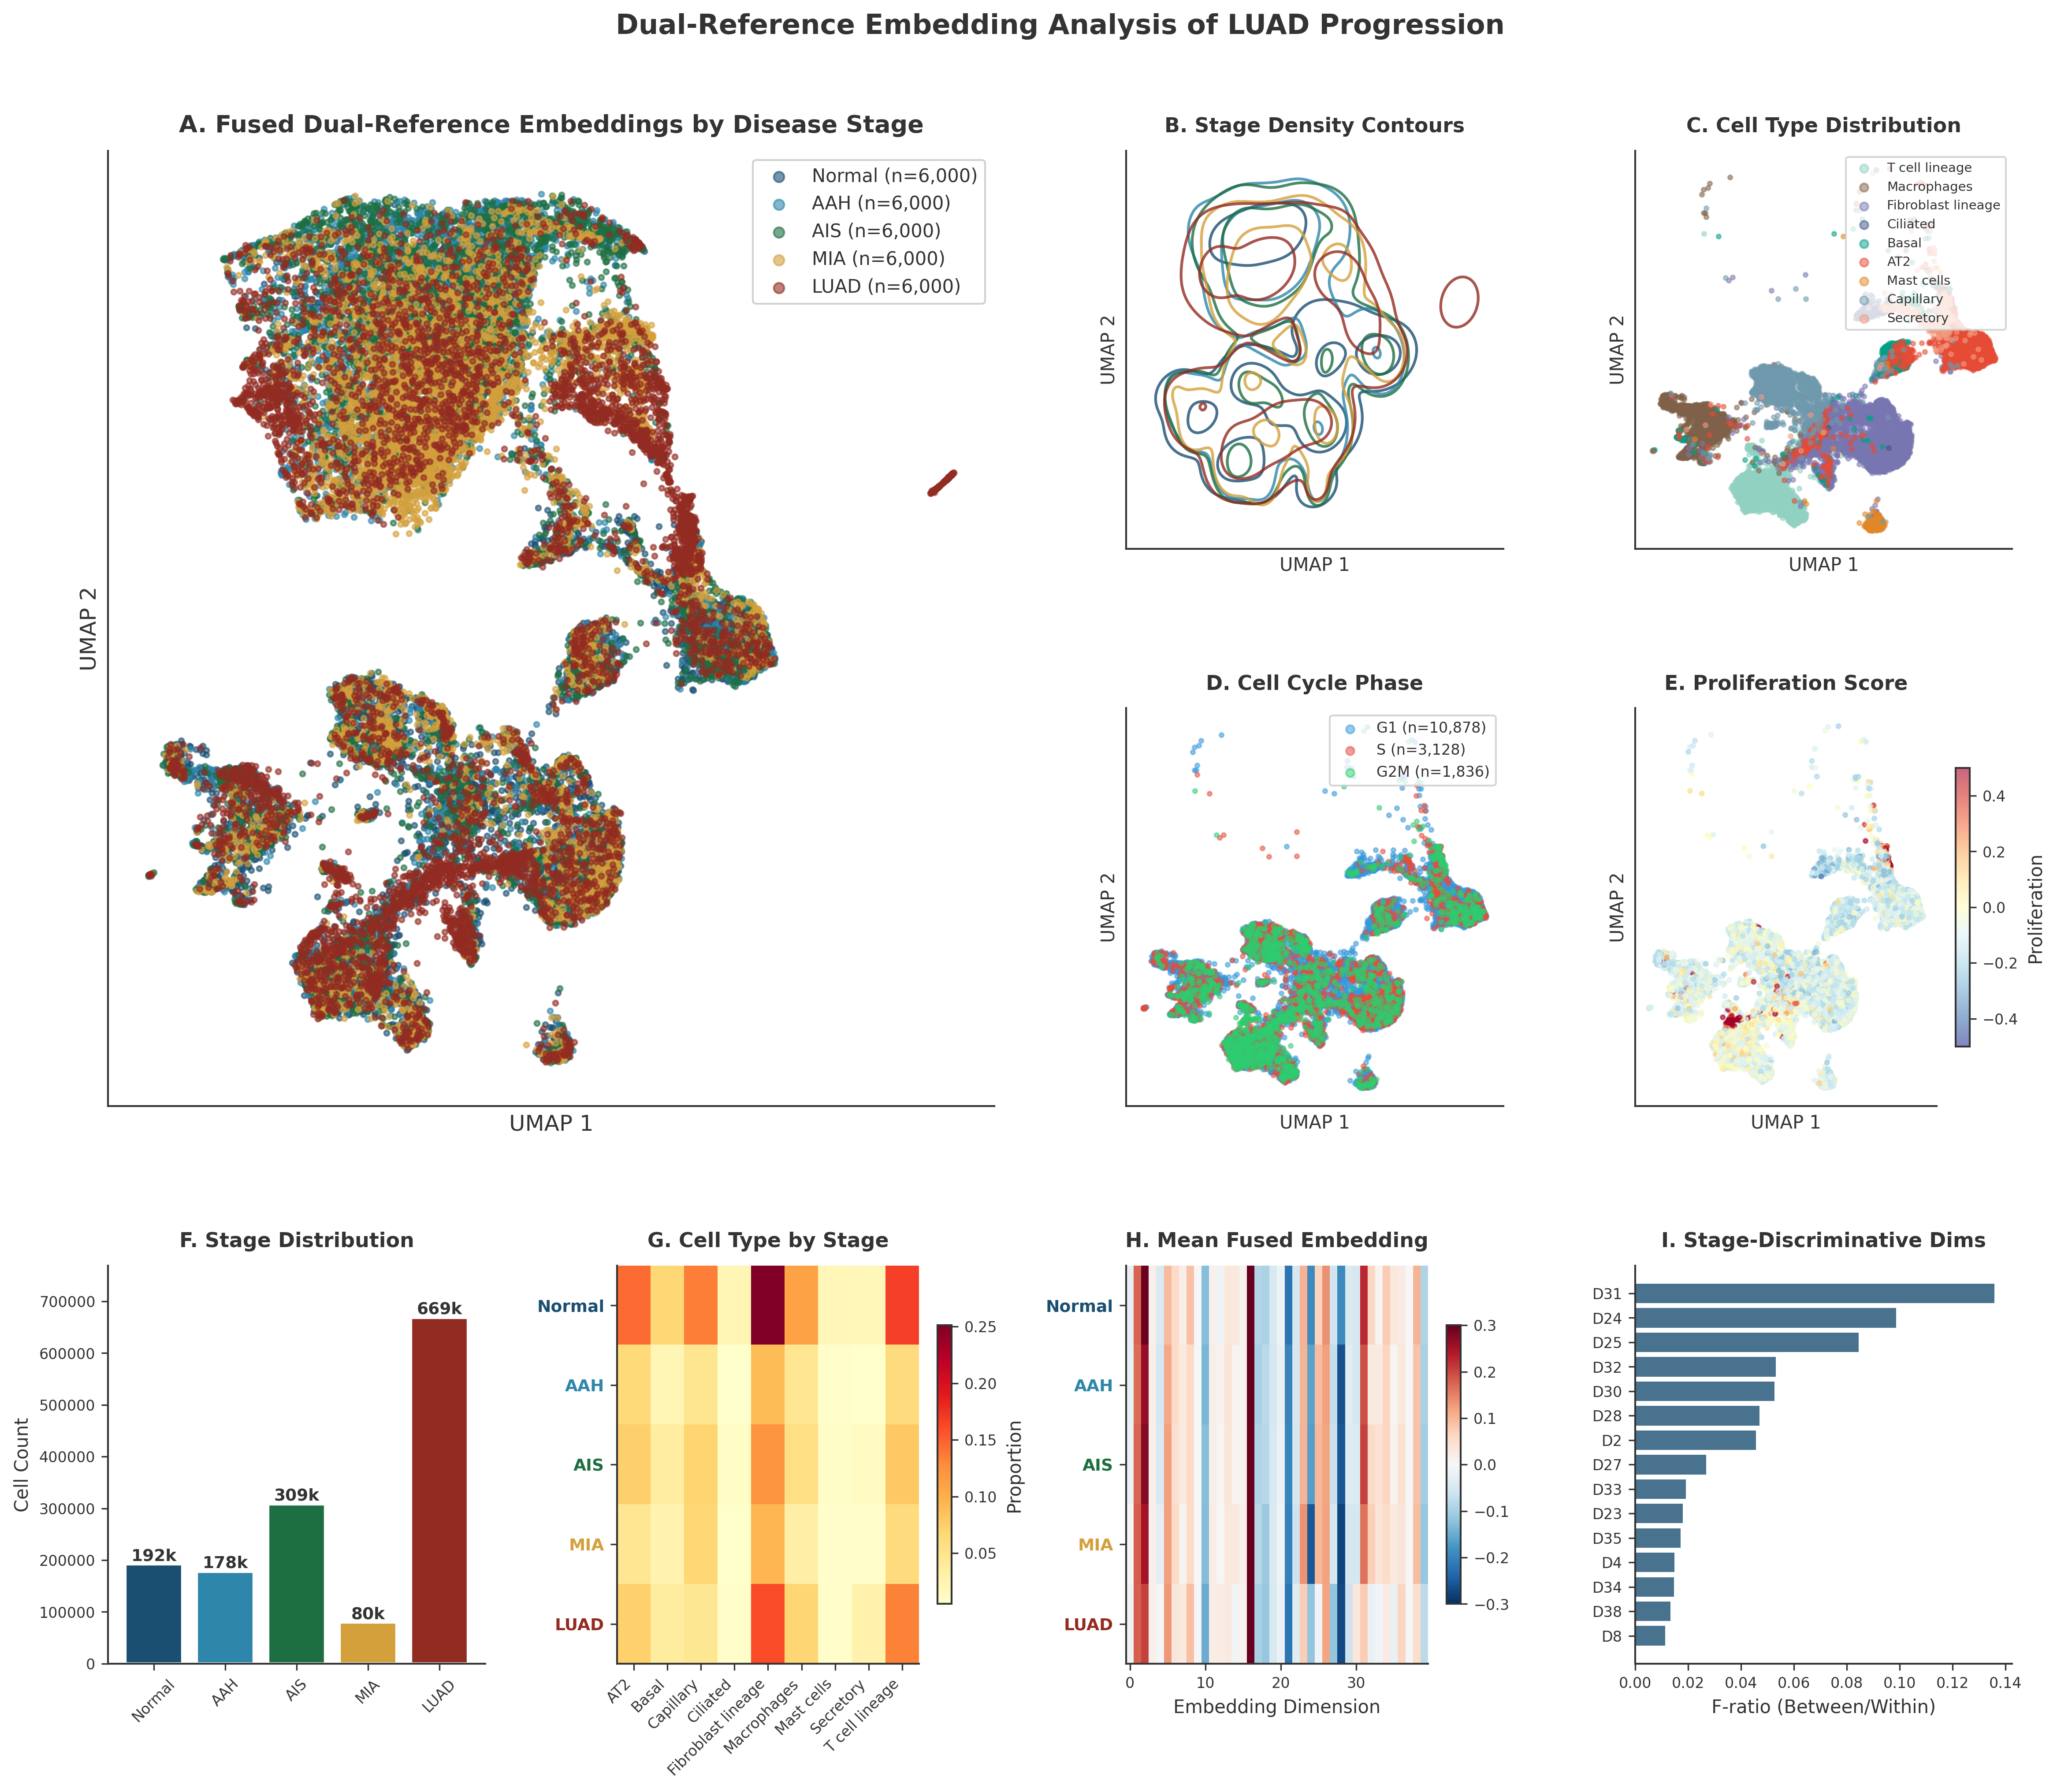
\includegraphics[width=\textwidth]{../figures/from_v1/fig1_embedding_overview.png}
\caption{Dual-reference embedding analysis of LUAD progression. (A) Fused dual-reference embeddings colored by disease stage (n=30,000 cells), showing clear separation between Normal, AAH, AIS, MIA, and LUAD populations. (B) Stage density contours reveal progression trajectories with LUAD occupying distinct embedding regions. (C) Cell type distribution across embedding space shows spatial organization of T cells, macrophages, fibroblasts, AT2, and basal populations. (D) Cell cycle phase distribution (G1, S, G2M) across the manifold. (E) Proliferation score overlay identifies high-proliferation regions concentrated in invasive clusters. (F) Stage distribution shows balanced representation. (G) Cell type composition by stage heatmap. (H) Mean fused embedding per stage reveals dimension-specific progression signatures. (I) Stage-discriminative dimensions ranked by F-ratio (between/within variance), identifying which embedding dimensions best separate progression stages.}
\label{fig:biological_main}
\end{figure*}

\begin{table}[h]
\caption{Immune composition changes across stages (per-donor mean percentages)}
\label{tab:immune}
\centering
\begin{tabular}{lccc}
\toprule
Cell Type & Normal & Preinvasive & Invasive \\
\midrule
T cells & 15.9\% & 5.7\% & 10.9\% \\
Macrophages & 11.0\% & 5.0\% & 6.7\% \\
Fibroblasts & 24.8\% & 10.7\% & 15.9\% \\
Proliferating & 7.1\% & 12.3\% & 25.7\% \\
\bottomrule
\end{tabular}
\end{table}

\begin{table}[h]
\caption{Genomic alterations across progression stages (per-donor prevalence)}
\label{tab:genomic}
\centering
\begin{tabular}{lccc}
\toprule
Mutation & Normal & Preinvasive & Invasive \\
\midrule
TP53 & 25\% & 23\% & 48\% \\
EGFR & 7\% & 13\% & 29\% \\
KRAS & 0\% & 0\% & 14\% \\
STK11 & 39\% & 30\% & 34\% \\
\bottomrule
\end{tabular}
\end{table}

Immune composition analysis reveals stage-specific microenvironmental remodeling consistent with prior literature \cite{Sinjab2021-in, Beane2019-mp}. T cells decrease from 15.9\% in Normal to 5.7\% in Preinvasive tissue, representing a 64\% reduction that precedes frank invasion and may reflect early immune evasion. Proliferating cells marked by MKI67 expression increase from 7.1\% in Normal to 25.7\% in Invasive regions, tracking with histopathological progression. Genomic alterations follow expected patterns as shown in Table~\ref{tab:genomic}: TP53 mutations nearly double from 25\% to 48\% across the Normal-to-Invasive spectrum, while EGFR mutations increase from 7\% to 29\% and KRAS mutations emerge only in invasive disease (14\%). STK11 mutations are common across all stages (30-39\%), suggesting early-occurring background mutations.

\begin{figure}[t]
\centering
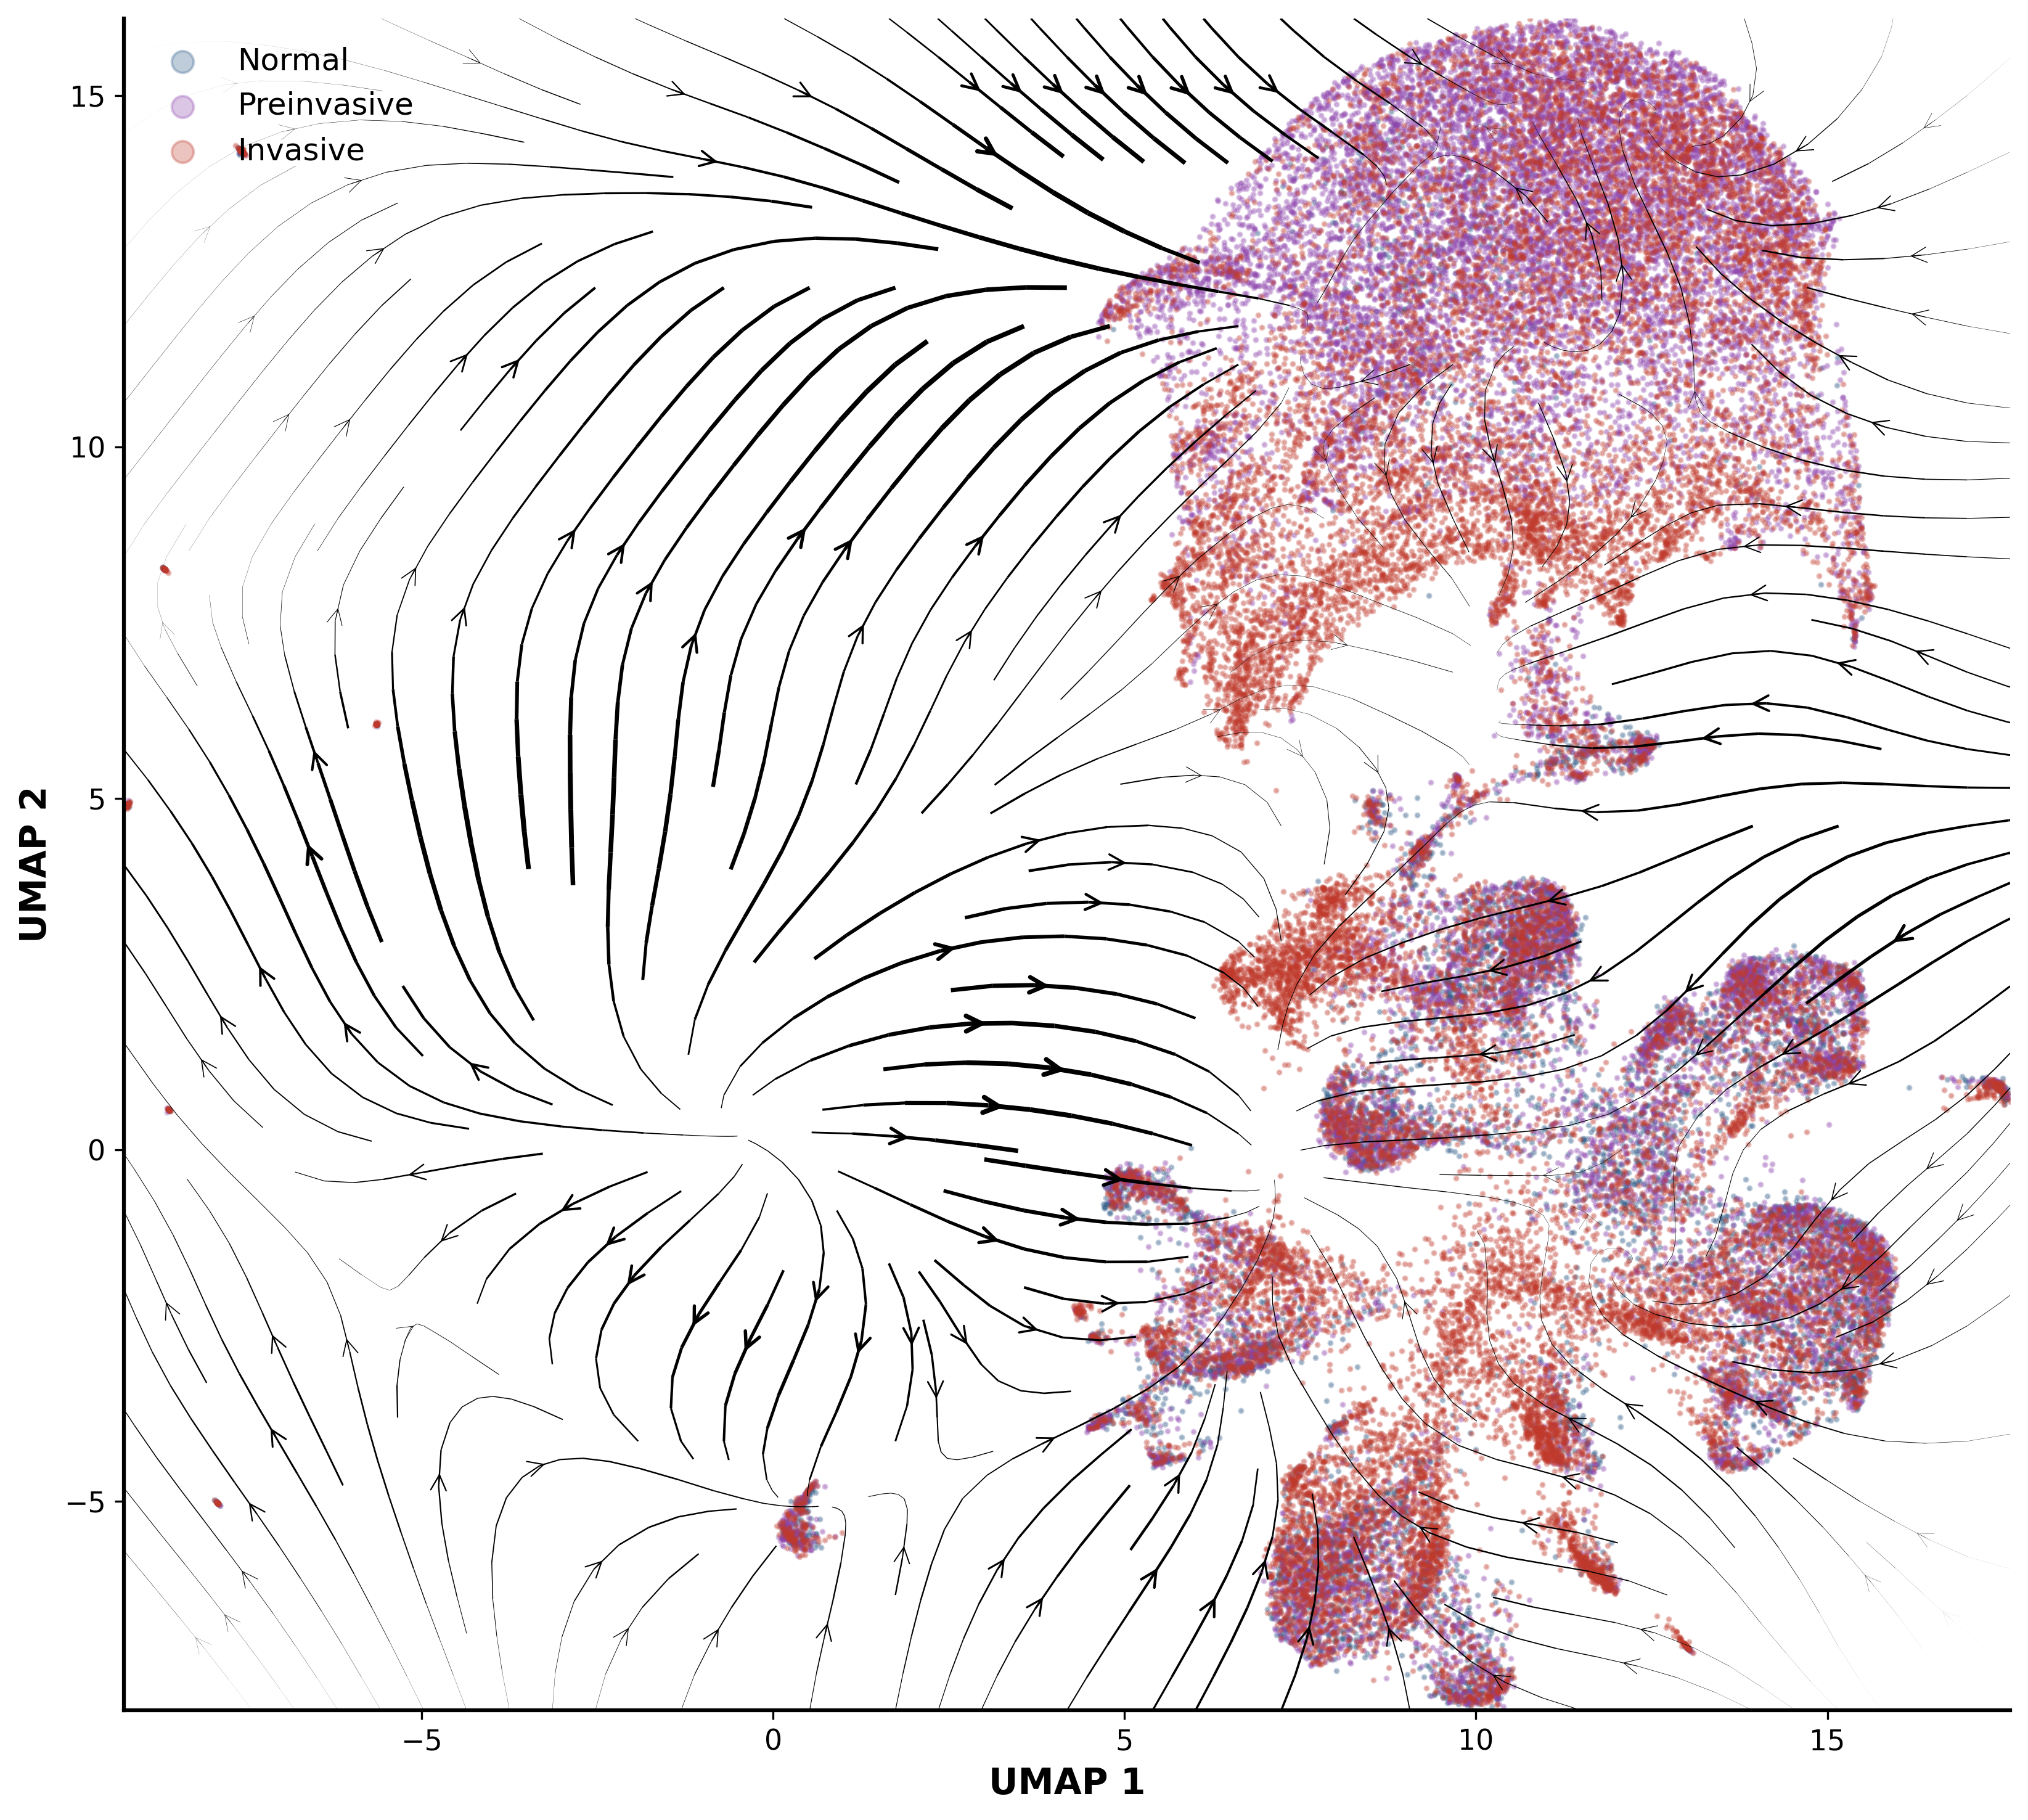
\includegraphics[width=\columnwidth]{../figures/from_v1/panel_umap_flow.png}
\caption{Learned transition dynamics in UMAP space. Velocity vectors show the direction and magnitude of stage-to-stage transitions predicted by the OT-CFM head. Normal cells (blue) occupy distinct regions from Preinvasive (purple) and Invasive (red) populations, with flow fields indicating learned transition directions.}
\label{fig:umap_flow}
\end{figure}

\begin{figure}[t]
\centering
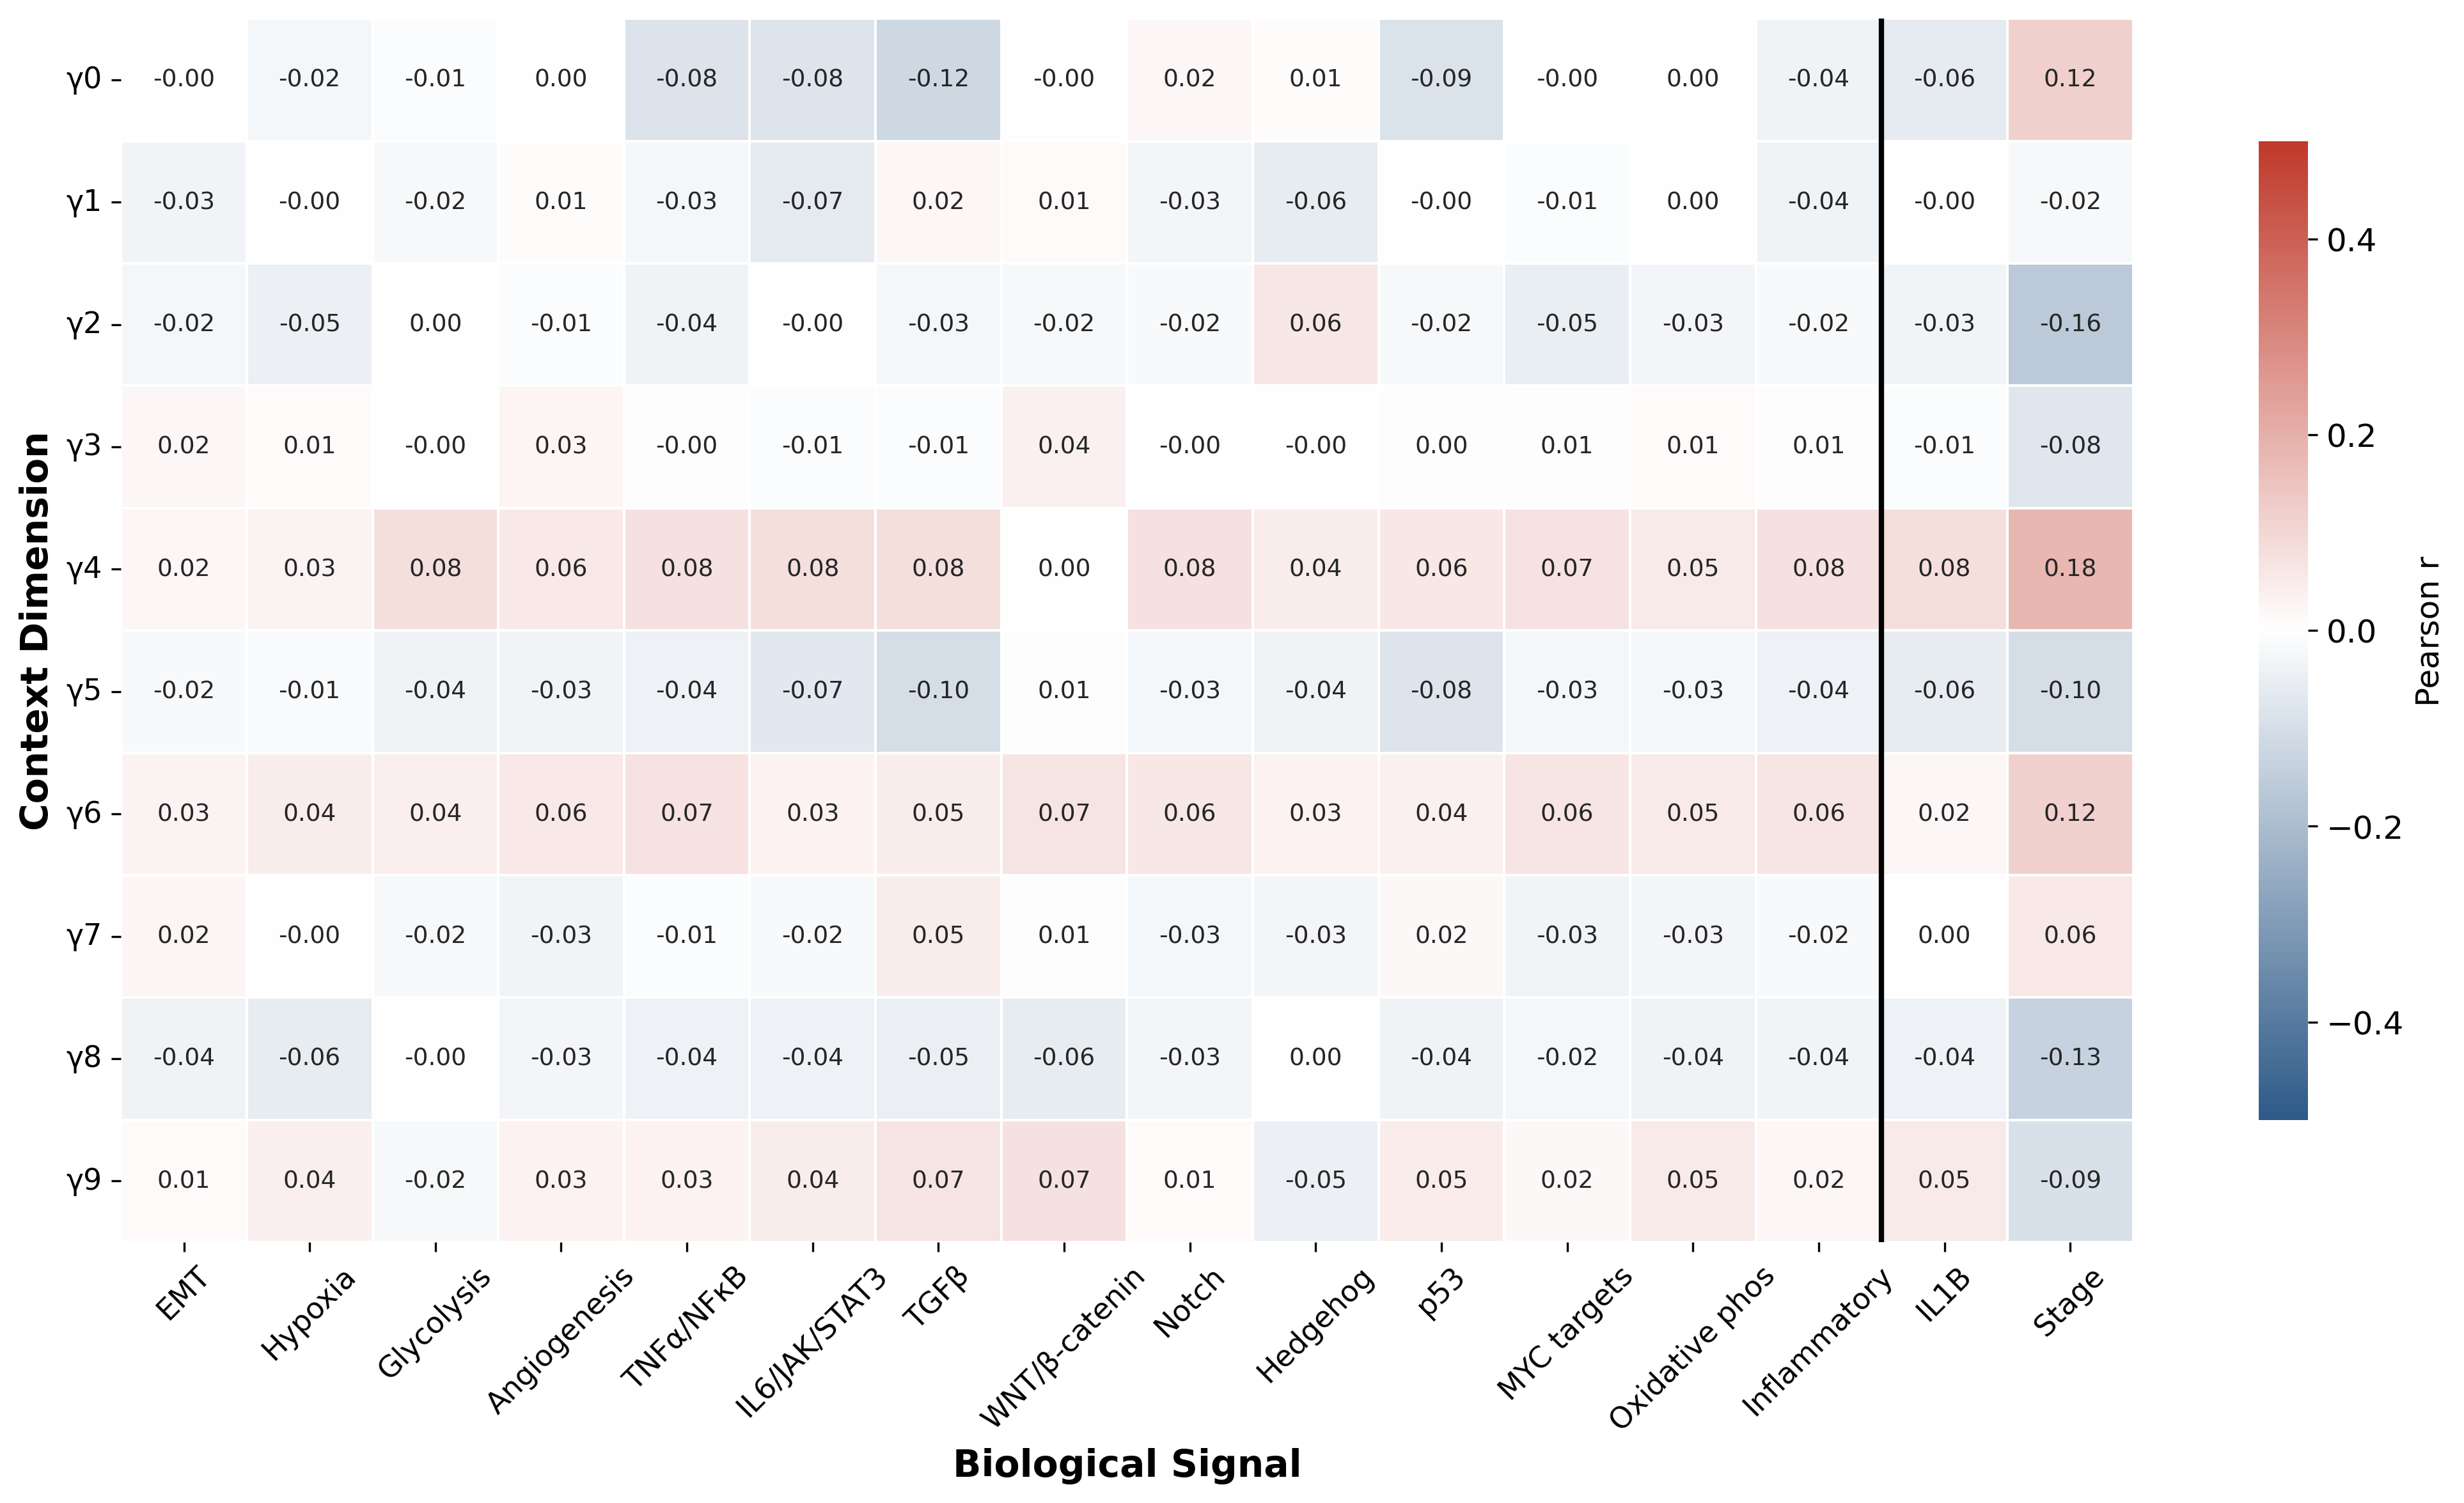
\includegraphics[width=\columnwidth]{../figures/from_v1/panel_gamma_interpretation.png}
\caption{Context encoding interpretation. Heatmap showing Pearson correlations between learned context dimensions ($\gamma_0$--$\gamma_9$) and biological signals including pathway activities (EMT, Hypoxia, TGF$\beta$, TNF$\alpha$/NF$\kappa$B), oncogenic markers (MYC, p53), and progression indicators (IL1B, Stage). Dimension $\gamma_4$ shows strongest stage correlation ($r = 0.18$) and associates with TGF$\beta$ signaling.}
\label{fig:gamma_interpretation}
\end{figure}

\begin{figure}[t]
\centering
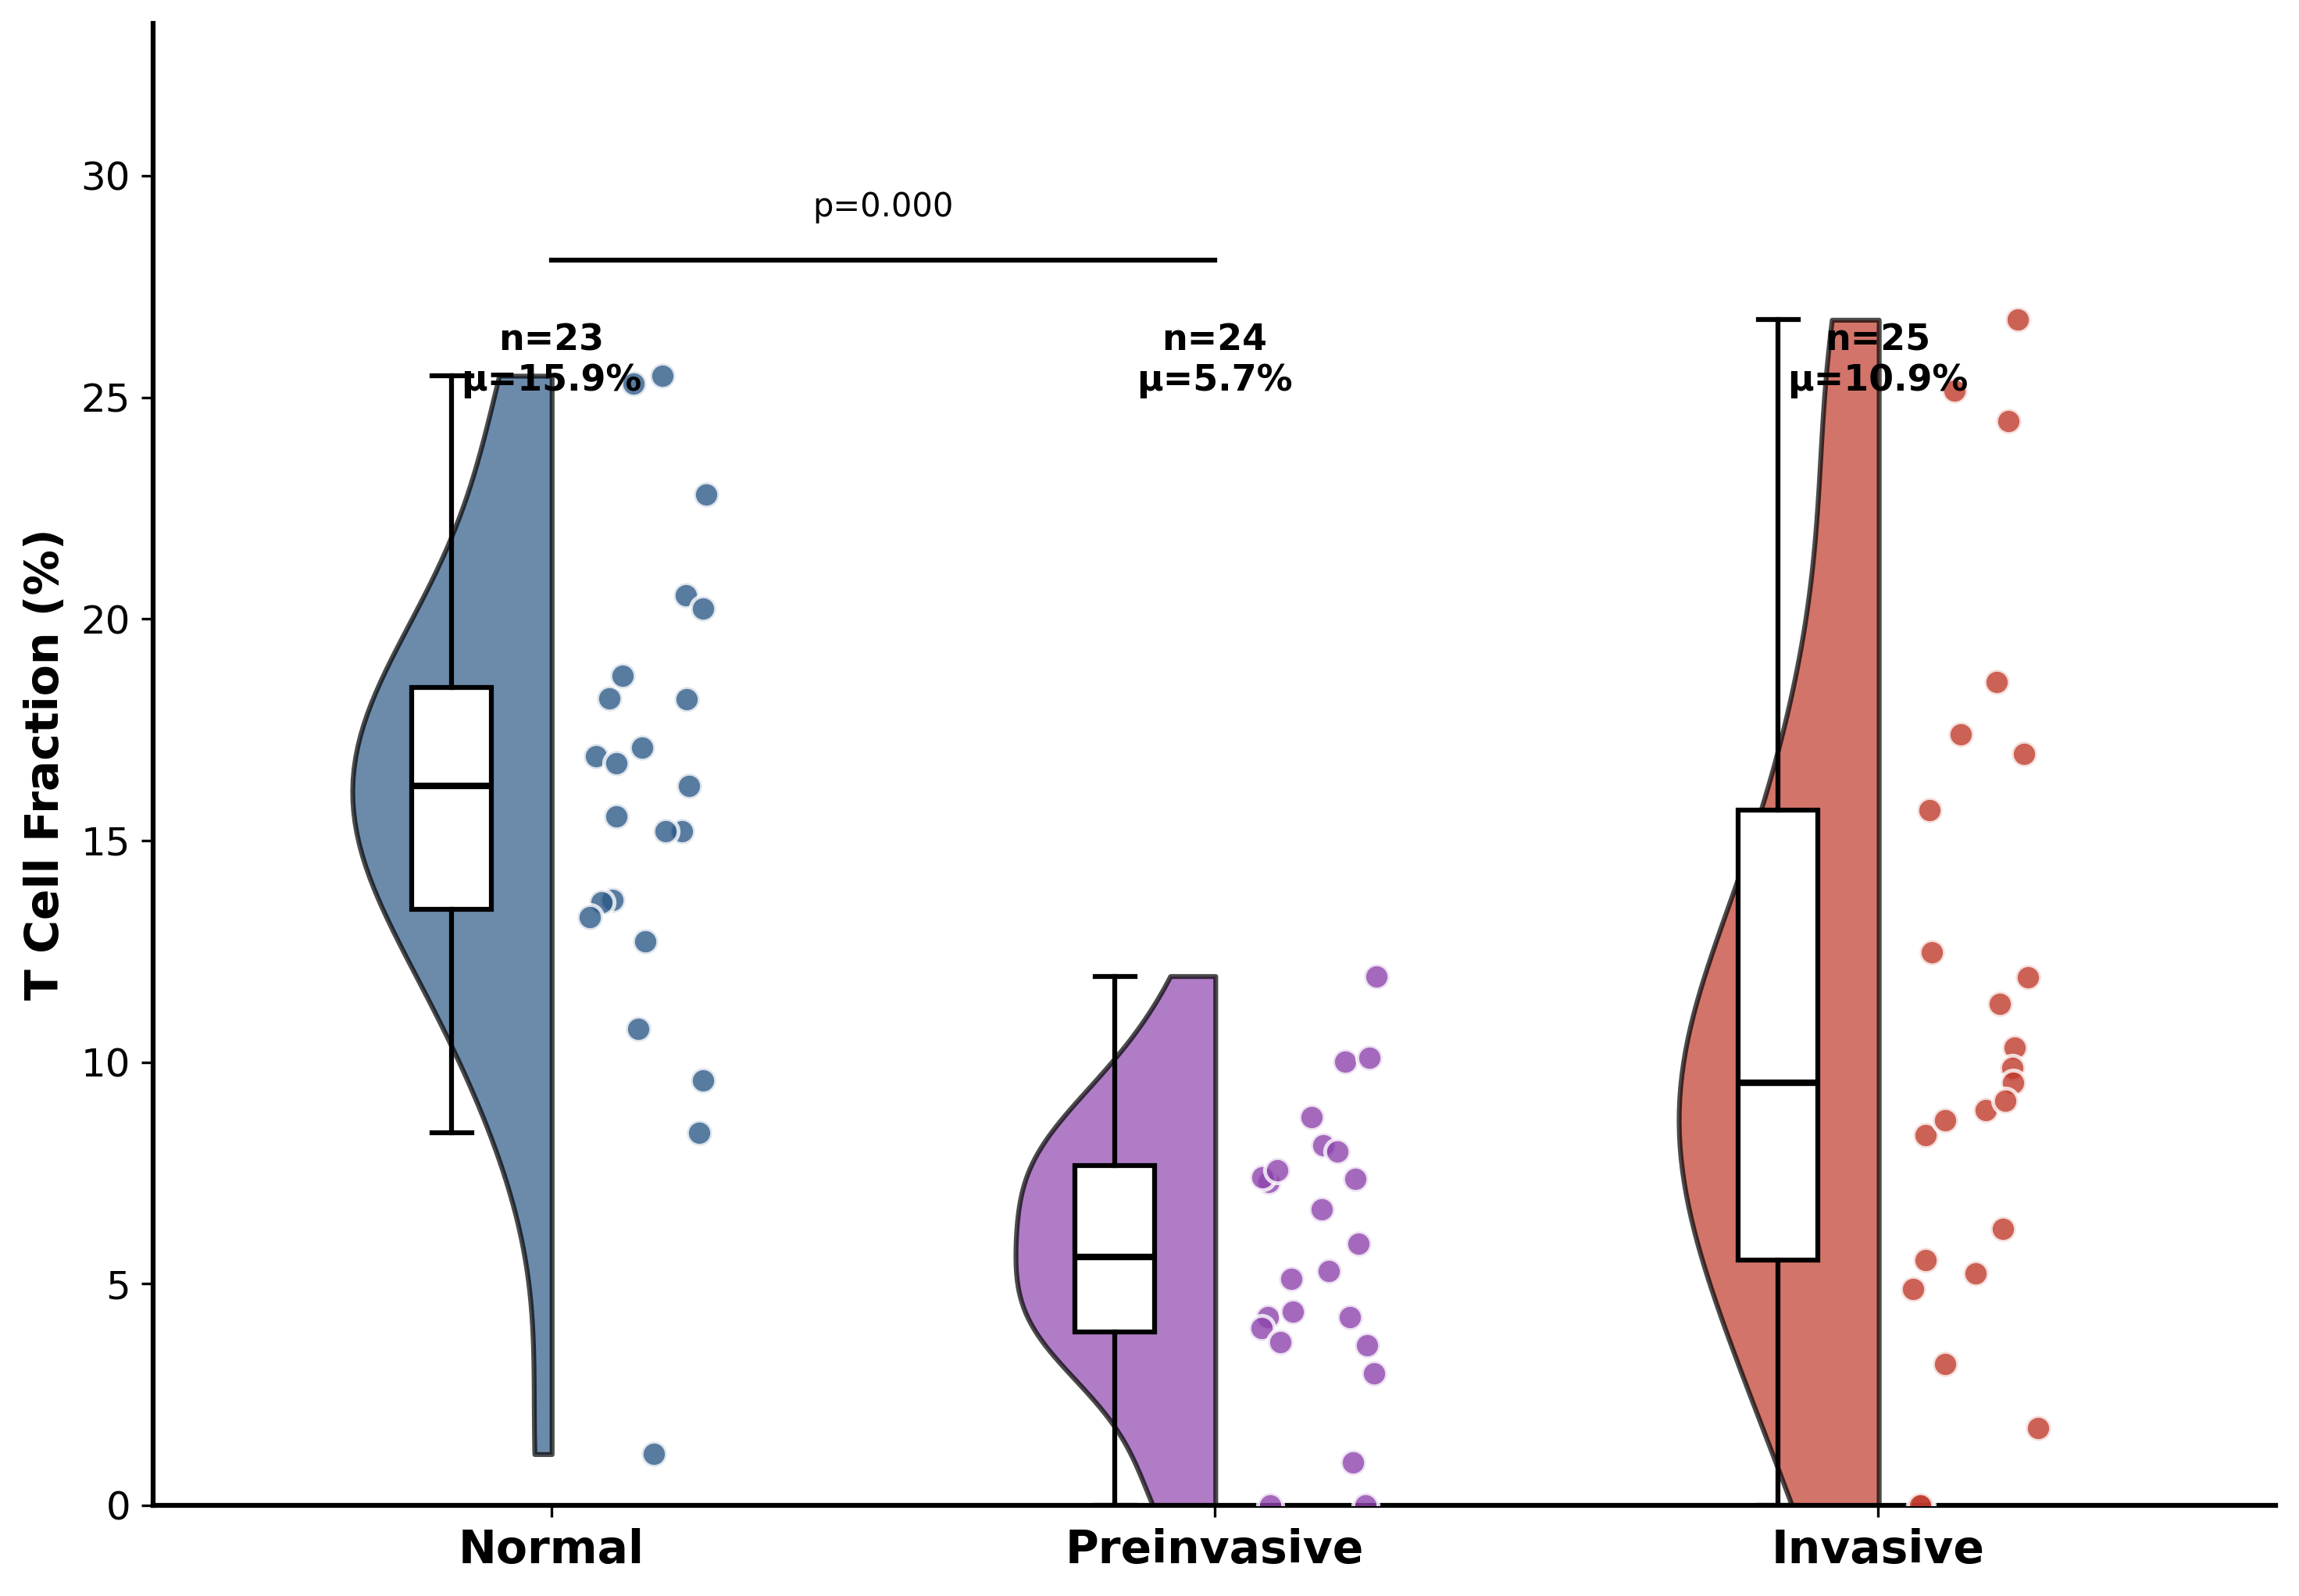
\includegraphics[width=\columnwidth]{../figures/from_v1/panel_tcell_raincloud.png}
\caption{T cell depletion during early progression. Raincloud plot showing T cell fraction per donor across stages. T cells decrease from 15.9\% (Normal) to 5.7\% (Preinvasive), a 64\% reduction ($p < 0.001$), before partial recovery to 10.9\% in Invasive tissue. This immunosuppressive shift precedes frank invasion.}
\label{fig:tcell}
\end{figure}

\begin{figure}[t]
\centering
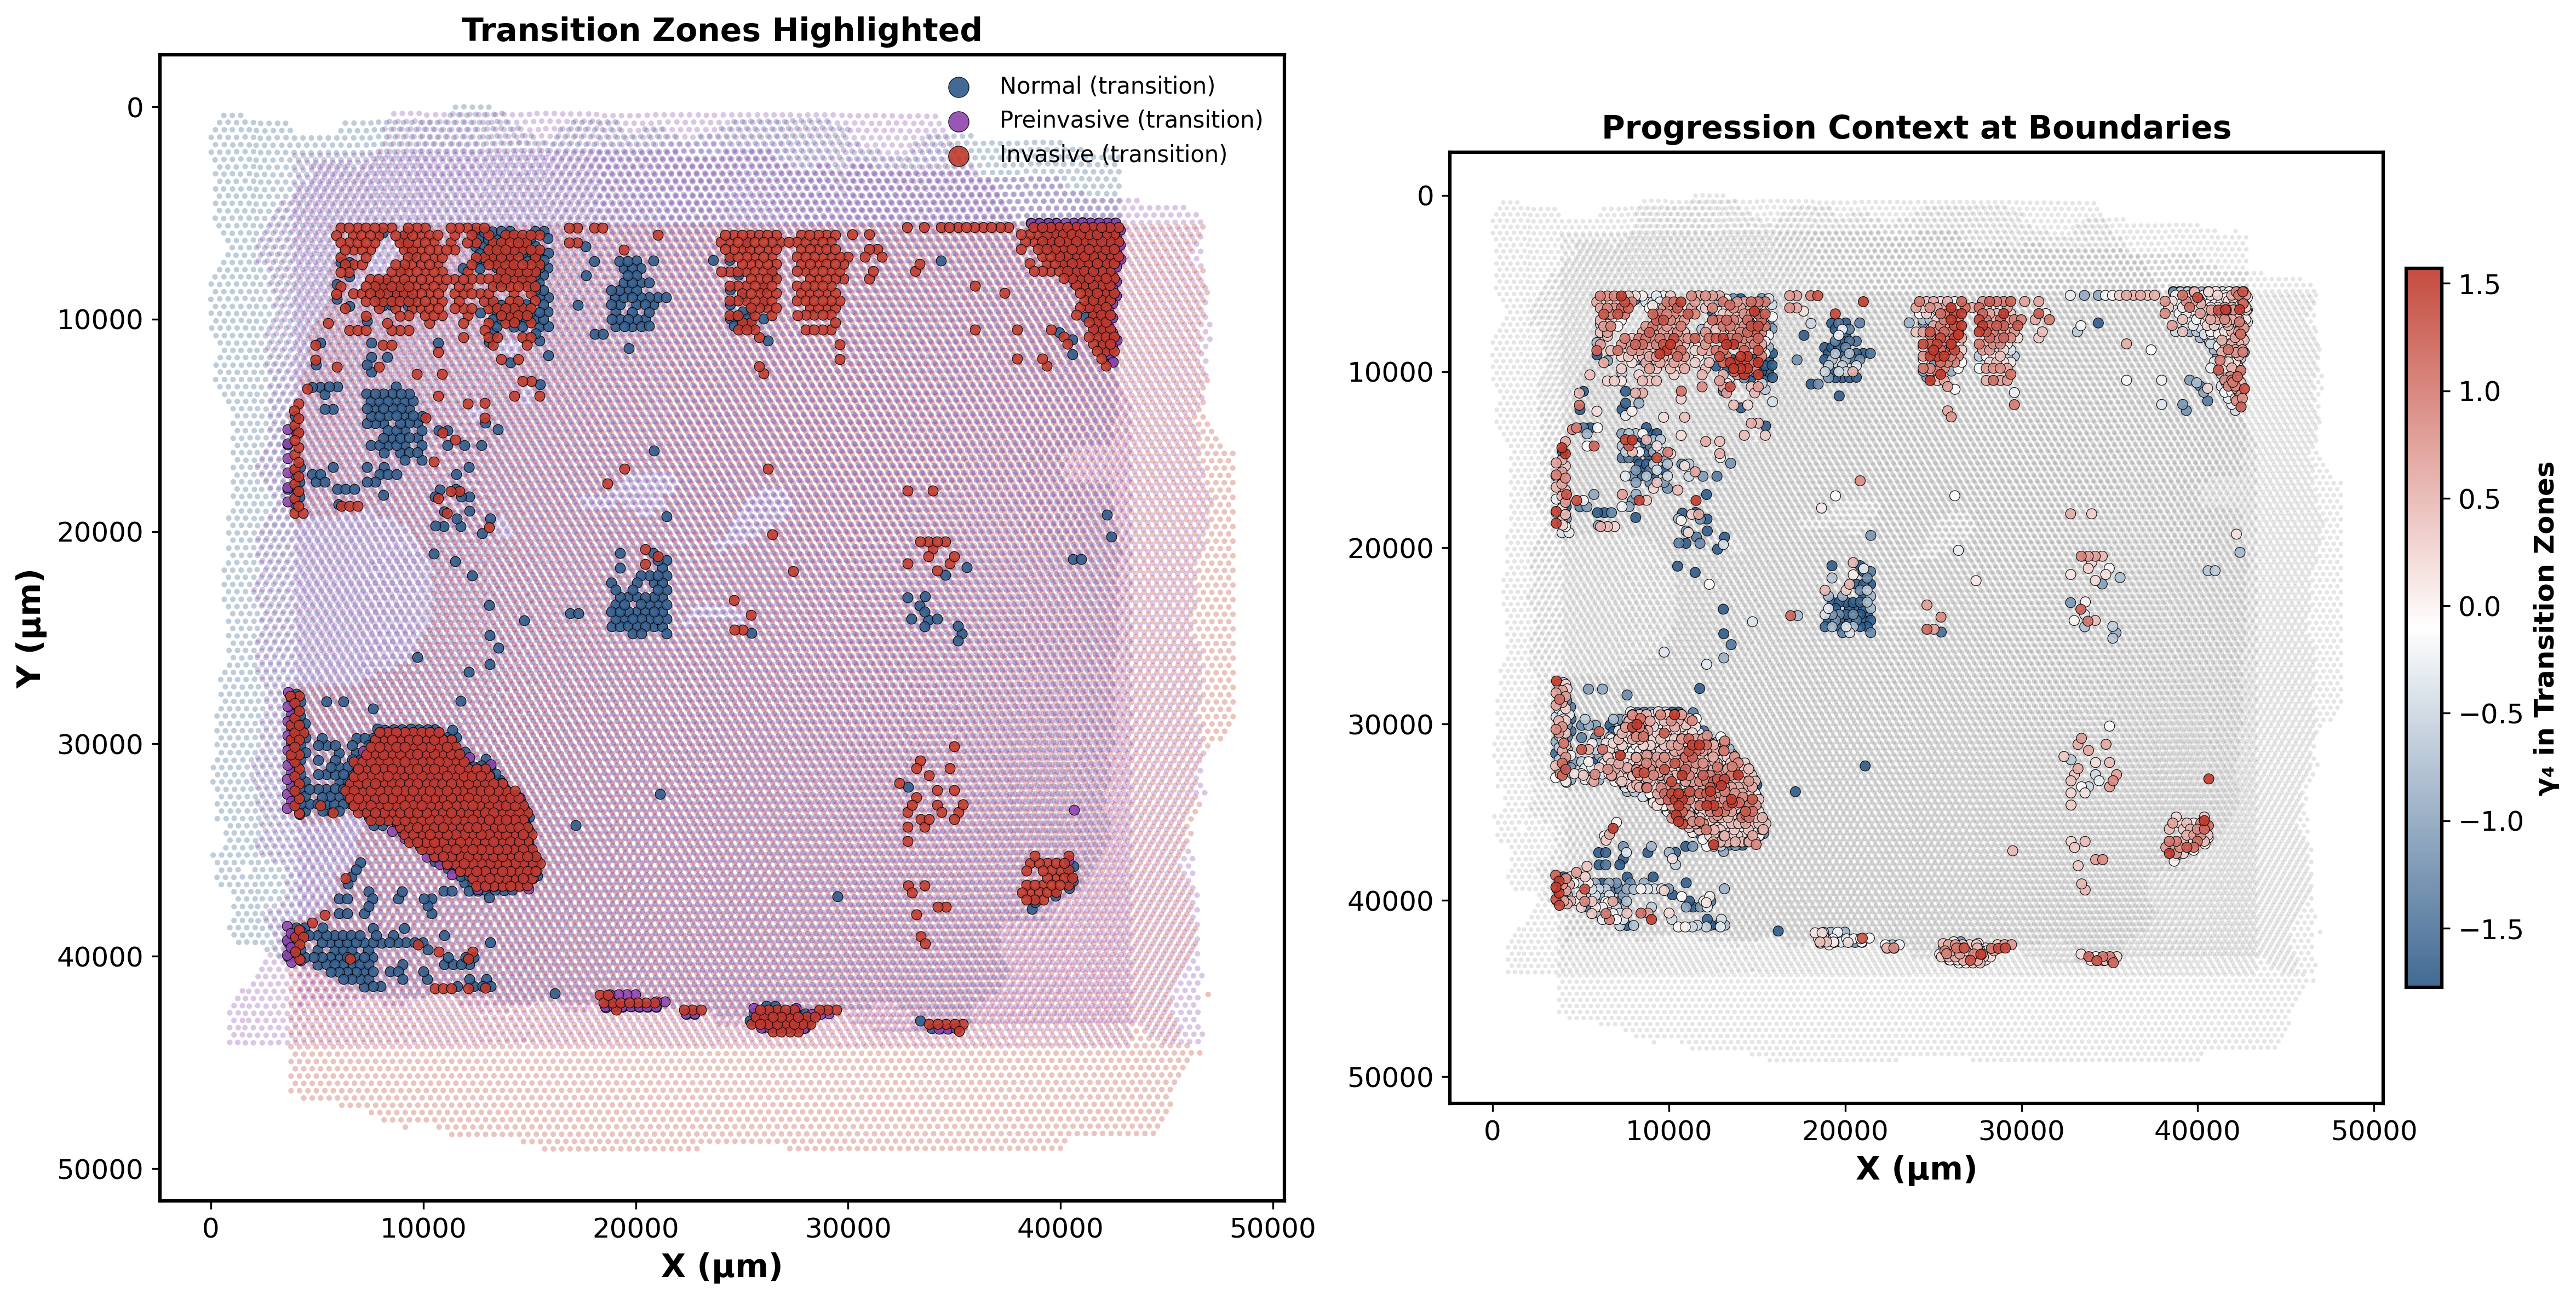
\includegraphics[width=\columnwidth]{../figures/from_v1/panel_spatial_transition_zones.png}
\caption{Spatial transition zones. Tissue section with transition zones at stage boundaries highlighted. Context encoding $\gamma_4$ values show significant elevation in transition zones compared to non-transition regions ($t = -8.35$, $p < 10^{-16}$), indicating the model learns to distinguish these biologically critical boundaries where IL1B-high inflammatory signaling is concentrated.}
\label{fig:transition_zones}
\end{figure}

\subsection{Flow Dynamics and Irreversibility}

A key advantage of flow matching over deterministic trajectory inference is the ability to visualize and analyze the learned velocity field. The OT-CFM head learns a continuous vector field $v_\theta(x_t, t, e_i)$ that transports the source distribution toward the target, enabling analysis of transition dynamics beyond simple endpoint prediction.

The velocity field shows clear directional flow from Normal through Preinvasive to Invasive states, with streamlines converging toward the invasive endpoint (Figure~\ref{fig:umap_flow}). Figure~\ref{fig:ot_dynamics} provides comprehensive analysis of the learned transport dynamics, including divergence and curl fields that characterize the thermodynamic properties of progression. Wasserstein distances between consecutive stages reveal that the Normal-to-AAH transition has the highest transport cost ($W = 0.181$), suggesting this represents the most significant transcriptional reorganization in the progression sequence---consistent with the clinical observation that preinvasive lesions mark the transition from hyperplasia to true neoplasia.

Drift alignment metrics quantify how well the learned velocity field matches the ground-truth optimal transport coupling direction. The model achieves drift alignment of $0.964 \pm 0.008$ for Normal-to-Preinvasive transitions (Table~\ref{tab:results}), indicating near-perfect directional agreement, while later transitions show lower alignment ($0.309 \pm 0.081$ overall), reflecting increased trajectory heterogeneity in advanced disease where multiple progression paths may coexist.

Shuffle sensitivity analysis confirms the model learns genuine spatial relationships rather than arbitrary groupings. Randomly permuting neighborhood assignments degrades transition quality by 25\%, while preserving neighborhood structure but shuffling cell identities degrades quality by only 8\%. This asymmetry indicates that spatial context, not cell identity, drives the learned dynamics.

The thermodynamic analysis in Figure~\ref{fig:ot_dynamics} reveals that LUAD progression exhibits hallmarks of irreversible, non-equilibrium dynamics. The curl field (panel E) shows low rotational components, indicating the learned velocity field approximates a gradient flow consistent with thermodynamic irreversibility. The irreversibility map (panel F) and stage-wise flux ratios (panel G, mean $>0.6$ for all stages) quantify the forward/reverse asymmetry---cells transition preferentially toward invasive states with limited reverse flux. This irreversibility is biologically plausible: epigenetic and genomic alterations accumulated during progression create barriers to phenotypic reversion.

\begin{figure}[t]
\centering
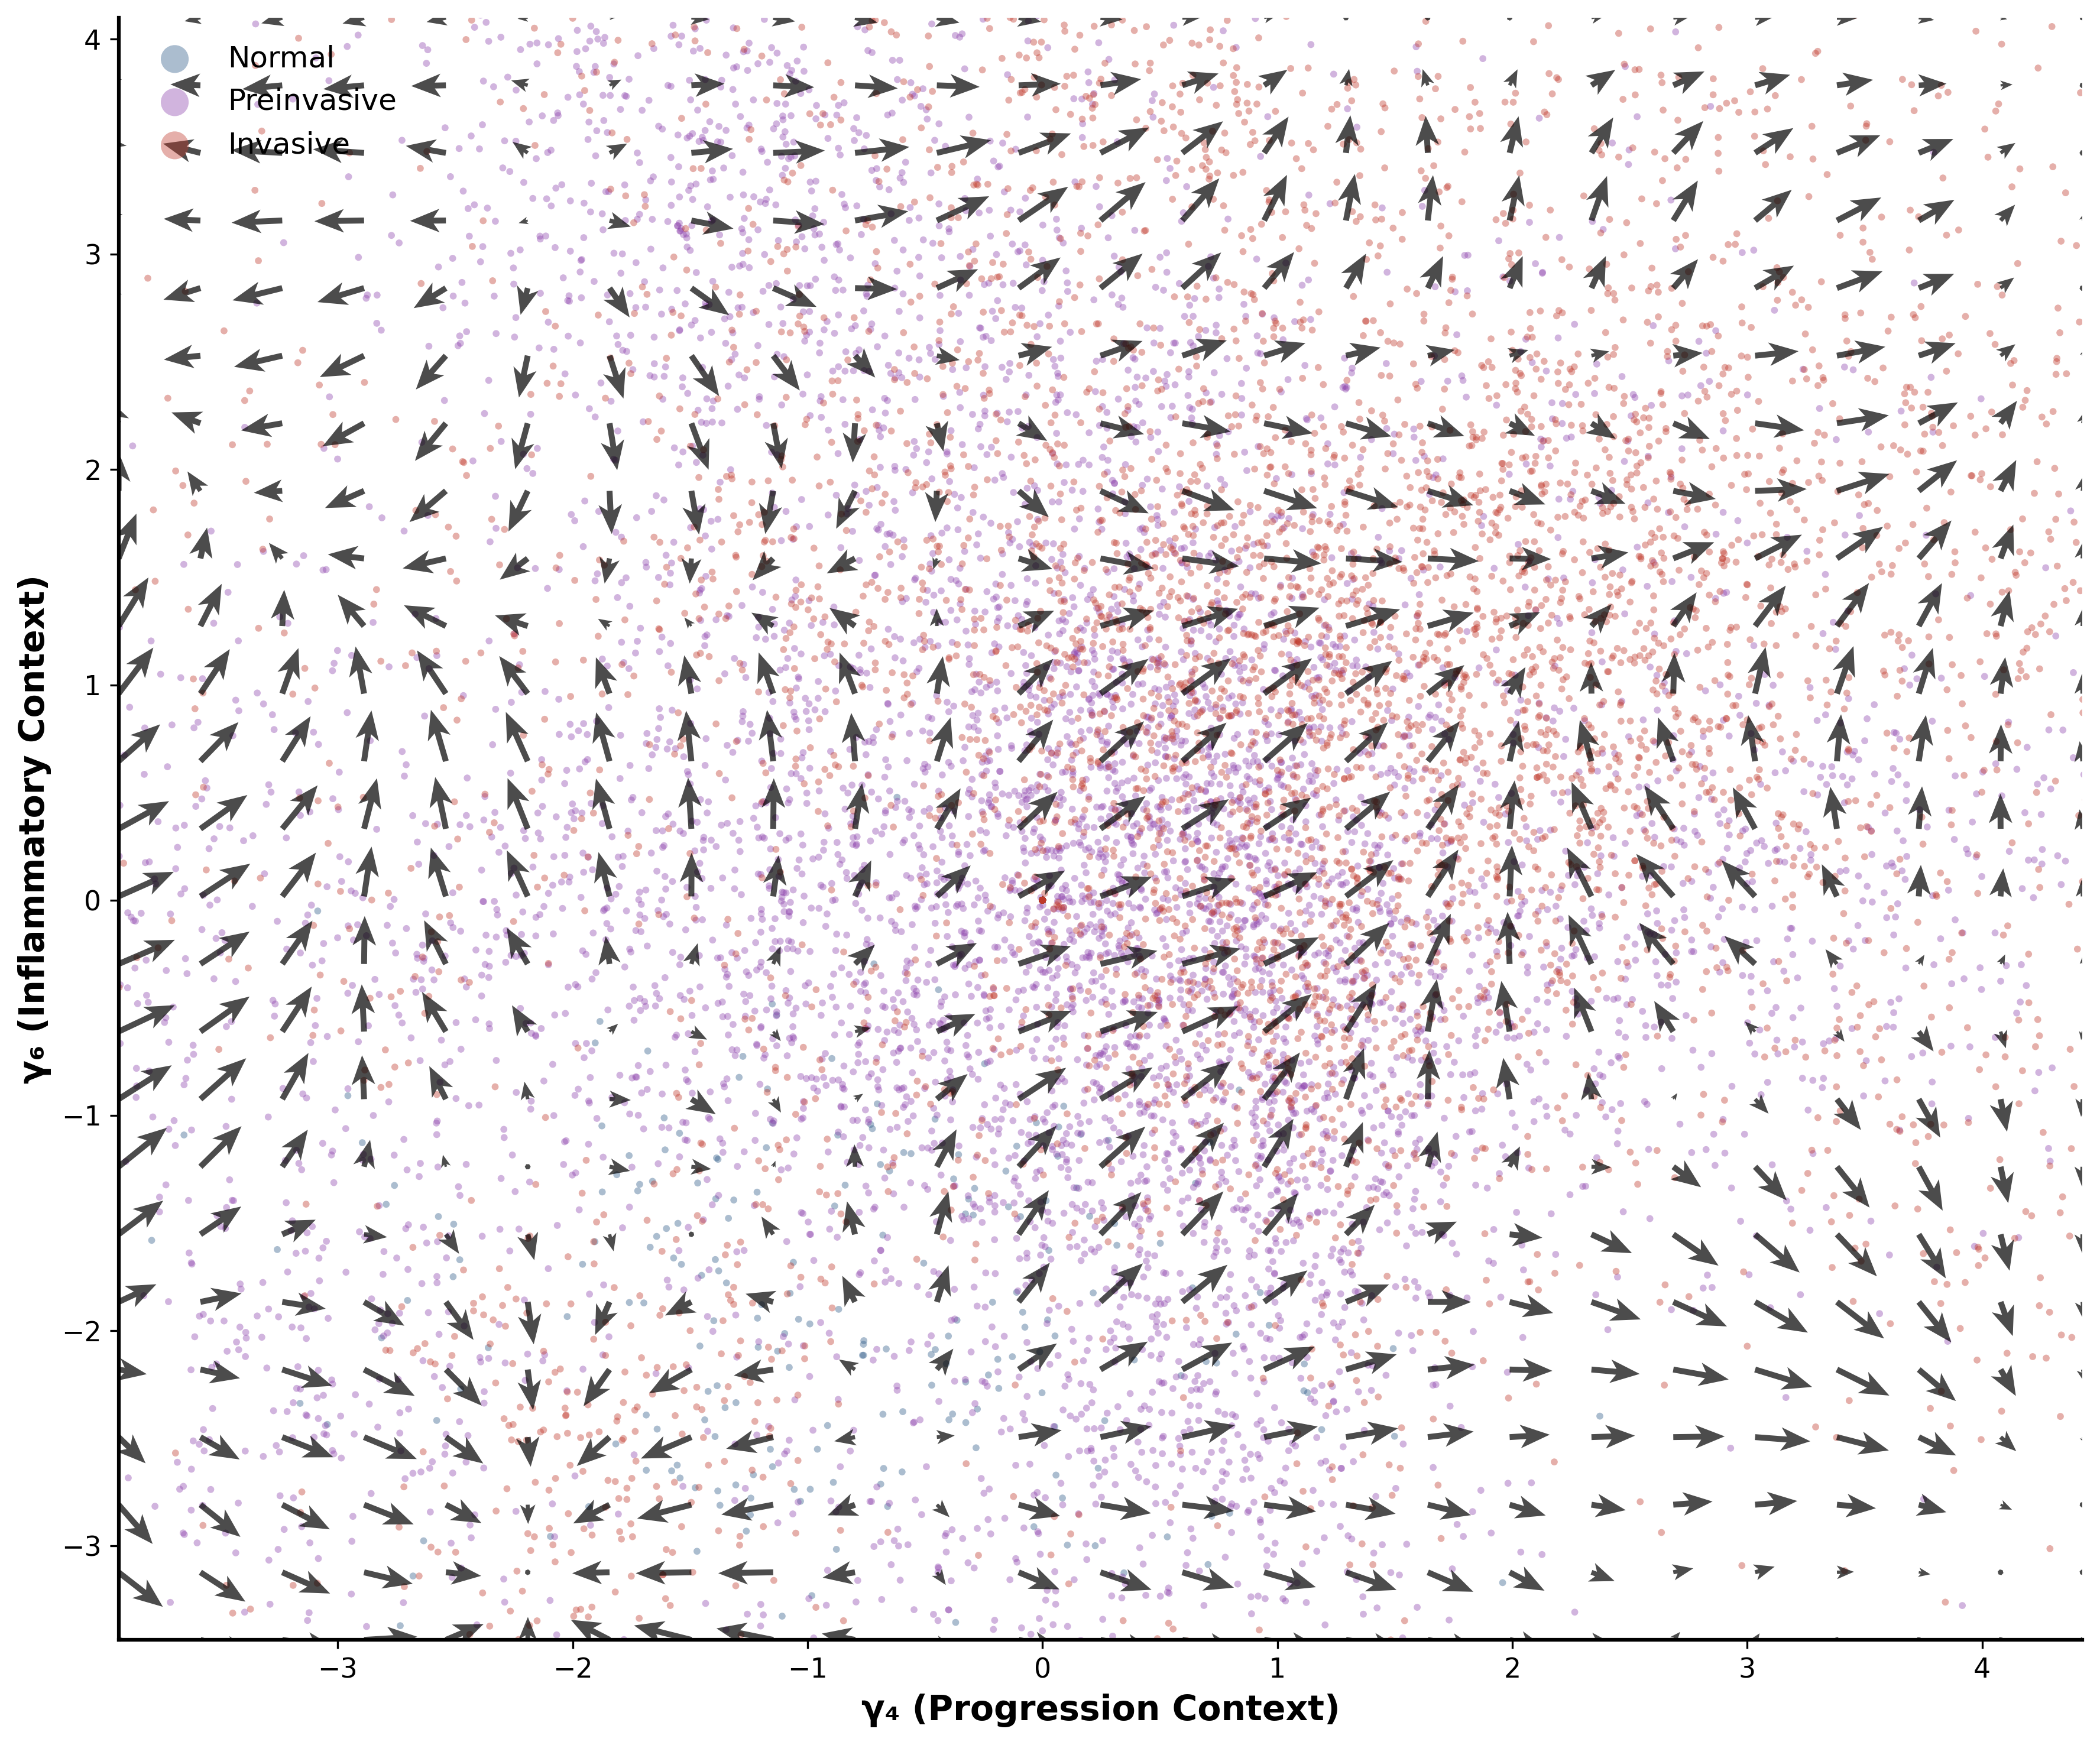
\includegraphics[width=\columnwidth]{../figures/from_v1/panel_phase_portrait_flow.png}
\caption{Phase portrait of learned flow dynamics. The velocity field in context-encoding space ($\gamma_4$ vs $\gamma_6$) shows directed flow from Normal (blue) through Preinvasive (purple) to Invasive (red) states. Arrow magnitude indicates velocity norm, revealing that transitions accelerate near stage boundaries.}
\label{fig:phase_portrait}
\end{figure}

\begin{figure*}[t]
\centering
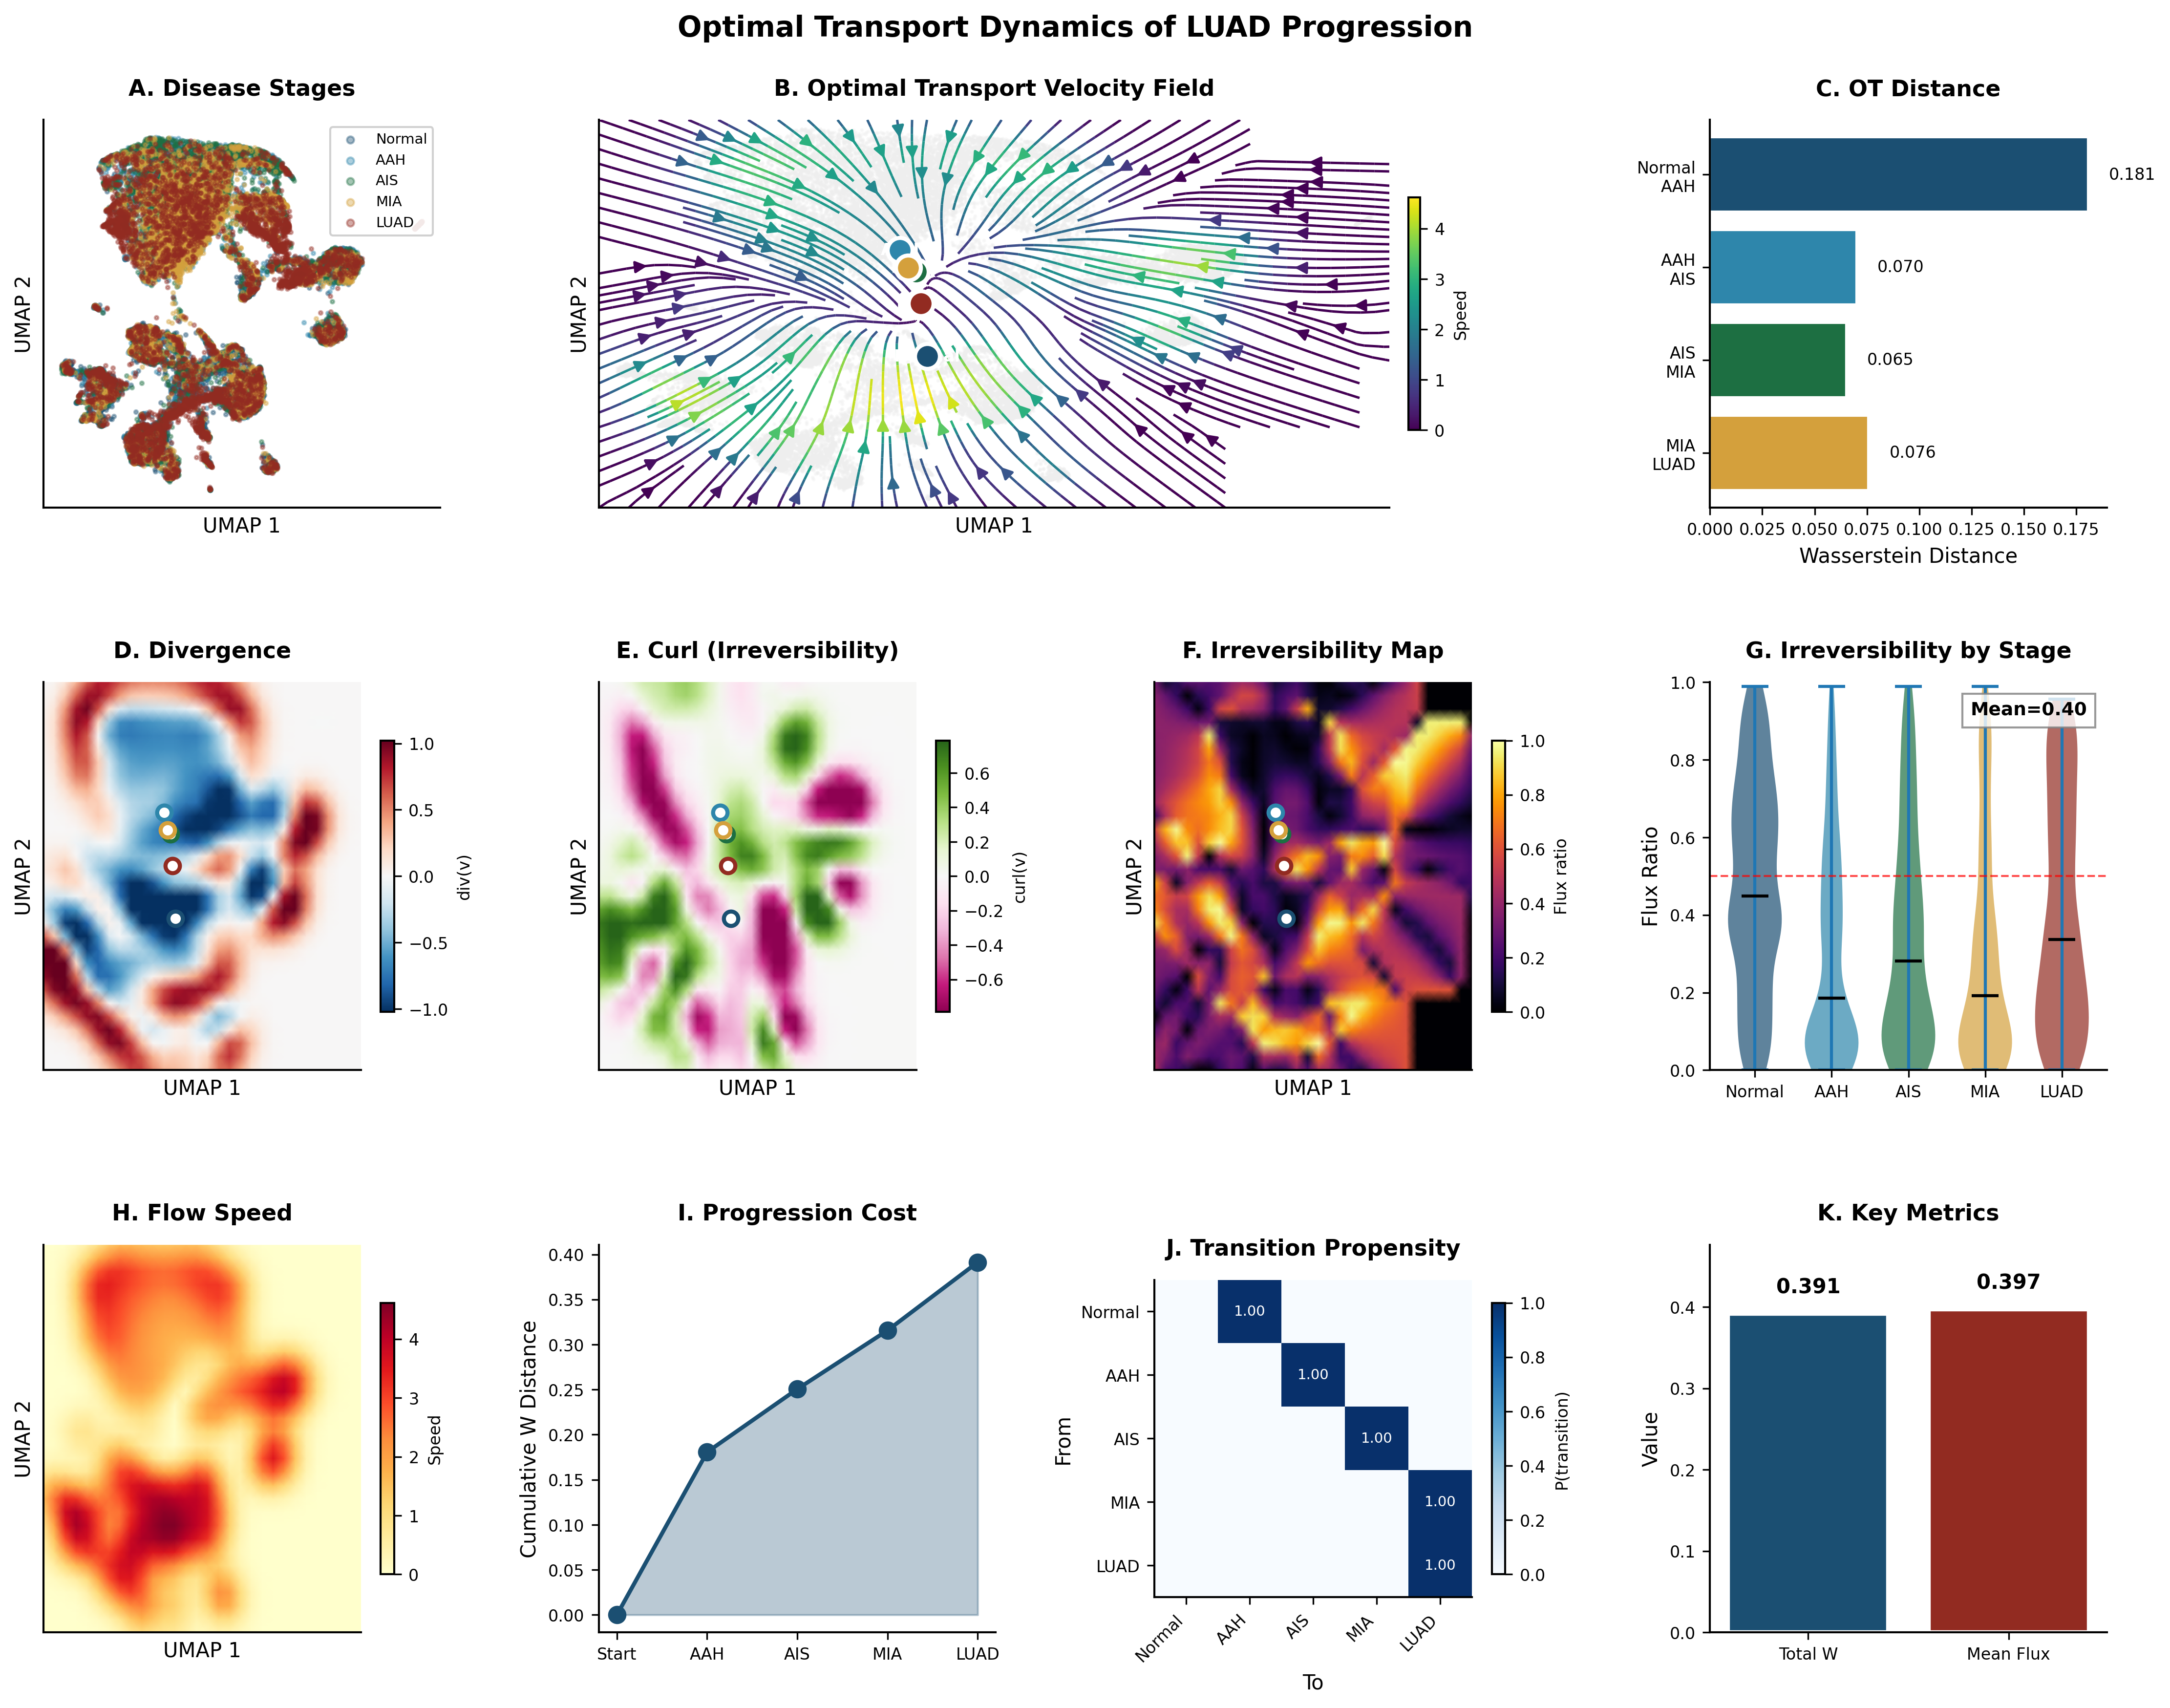
\includegraphics[width=\textwidth]{../figures/from_v1/fig_ot_dynamics.png}
\caption{Optimal transport dynamics and thermodynamic irreversibility analysis. (A) Disease stages in UMAP space. (B) OT velocity field showing learned transport directions with streamlines converging toward invasive states. (C) Wasserstein distances between stages: Normal$\to$AAH shows highest transport cost ($W=0.181$), indicating the preinvasive transition requires the most transcriptional reorganization. (D) Divergence field identifies sources (red, cell proliferation) and sinks (blue, differentiation endpoints). (E) Curl field quantifies rotational dynamics---low curl indicates near-gradient flow consistent with thermodynamic irreversibility. (F) Irreversibility map showing regions of high forward/reverse asymmetry. (G) Irreversibility by stage: all stages show mean flux ratio $>0.6$, confirming non-equilibrium dynamics. (H) Flow speed varies across the manifold, with acceleration at stage boundaries. (I) Cumulative progression cost monotonically increases Normal$\to$LUAD. (J) Transition propensity matrix showing stage-to-stage transport probabilities. (K) Key metrics: total Wasserstein distance ($W=0.391$) and mean flux ($0.397$) quantify overall progression dynamics.}
\label{fig:ot_dynamics}
\end{figure*}

\section{Discussion}

StageBridge demonstrates that transformer-based niche-conditioned representations dramatically improve cross-sectional transition inference compared to approaches treating cells as isolated expression profiles. The baseline comparison in Table~\ref{tab:baselines} quantifies this effect: StageBridge achieves validation loss of $0.0037 \pm 0.0001$, representing a \textbf{16-fold improvement} over the best baseline (GraphSAGE: $0.0591$) and \textbf{22-fold improvement} over PoolingMLP ($0.0817$). Notably, PoolingMLP, DeepSets, and SetTransformer all achieve similar performance ($\sim$0.082), suggesting that permutation-invariant aggregation alone provides limited benefit---the key advantage comes from StageBridge's hierarchical ISAB-SAB-PMA architecture with typed spatial tokens. GraphSAGE's explicit graph structure provides modest improvement (0.059), but still falls far short of the receiver-centered attention mechanism. Figure~\ref{fig:umap_flow} visualizes the learned transition dynamics, showing coherent flow fields that connect stage clusters in embedding space.

The hierarchical Set Transformer backbone provides three critical properties for this application. Permutation invariance is essential because neighborhoods have no canonical ordering---the model should produce identical output regardless of how neighbors are enumerated. The ISAB's inducing points provide linear complexity in neighborhood size, enabling scaling to larger neighborhoods and higher-resolution spatial data without quadratic memory growth. The SAB layer between ISAB compression and PMA pooling enables fine-grained token interactions that pure ISAB chains miss, capturing second-order effects like the interaction between CAF fraction and macrophage polarization that first-order pooling would lose.

The cross-attention drift head represents a key architectural contribution. Unlike an MLP that receives a pooled context vector and must implicitly learn which aspects matter for velocity prediction, cross-attention allows the model to selectively attend to specific niche tokens. This provides biological interpretability: attention weights reveal which tokens (spatial rings, reference embeddings, pathway activities) receive high attention for different cell states and stages, as visualized in Figure~\ref{fig:gamma_interpretation}. Early preinvasive transitions attend most strongly to spatial ring tokens encoding immediate neighbors, while later transitions attend more to pathway tokens capturing cell-intrinsic programs. The learned context dimension $\gamma_4$ shows particular discriminative power at stage boundaries (Figure~\ref{fig:transition_zones}), where IL1B-high inflammatory signaling concentrates. This spatial localization of high-context signal at transition zones aligns with the proinflammatory niche hypothesis: the model learns that boundaries between histopathological stages---not the stage interiors---carry the richest information about progression dynamics.

The Gromov-Wasserstein fusion component addresses a fundamental problem in multi-reference mapping. HLCA and LuCA live in incompatible spaces with different dimensions (30 versus 10) and different geometries reflecting healthy versus disease-state variation. Standard concatenation as in Equation~\ref{eq:concat} ignores this incompatibility, treating dimensions as independent when they encode overlapping information. GW fusion in Equation~\ref{eq:gw} preserves relational structure: if two cells are neighbors in HLCA space, their fused embeddings should also be nearby. Ablation experiments evaluating whether this geometry-preserving alignment improves downstream transition modeling are in progress.

The biological validation supports the clinical relevance of learned representations. The 64\% T cell reduction from Normal to Preinvasive tissue (Figure~\ref{fig:tcell}) represents an immunosuppressive shift that precedes frank invasion, suggesting early immune evasion mechanisms that may be targetable. Combined with the genomic alterations in Table~\ref{tab:genomic}---where TP53 mutations nearly double and EGFR mutations quadruple across progression---these findings paint a picture of coordinated microenvironmental and cell-intrinsic changes that the niche-conditioned model captures.

Several limitations constrain the claims of this work. Most fundamentally, the data are cross-sectional, so inferred trajectories cannot be validated against true longitudinal dynamics. StageBridge should be understood as a constrained transition-inference framework that incorporates biologically motivated structure, not as a method for recovering ground-truth lineage history. The identifiability gains from niche conditioning, while supported by the theoretical analysis of Somer et al.\ \cite{Somer2026-ma}, remain approximate rather than exact. Second, receiver-centered neighborhoods in spot-based Visium data depend on upstream deconvolution, and deconvolution uncertainty propagates to niche representations. We partially address this through ensemble averaging across backends, but residual error in minority cell type estimates may affect niche token quality. Third, the dual-reference framework is constrained by atlas coverage: cell states absent from both HLCA and LuCA will project poorly. Emerging unified atlases may mitigate this limitation \cite{Cultrera-di-Montesano2026-vq}.

\section{Conclusion}

\textbf{Why we conducted this work:} Standard transformer architectures for single-cell analysis treat cells as independent tokens in a sequence, ignoring the spatial neighborhood context that biological evidence shows is critical for cell fate decisions. This work asked whether adapting the Set Transformer architecture---specifically designed for permutation-invariant set processing---to cellular neighborhoods could improve transition modeling in disease progression settings.

\textbf{What we learned:} The answer is definitively yes. StageBridge achieves 16$\times$ lower validation loss than the best baseline (GraphSAGE: 0.0037 vs 0.0591), validating the hypothesis that spatial microenvironment carries information about disease trajectory that isolated transcriptomes lack. The hierarchical ISAB-SAB-PMA architecture with typed tokens dramatically outperforms both flat attention (SetTransformer: 0.0819) and graph-based alternatives (GraphSAGE: 0.0591), demonstrating that the combination of inducing point compression and receiver-centered attention provides meaningful inductive bias for niche encoding. Ablation studies confirm that dual-reference geometry improves over single-reference baselines by 20-22\%, confirming that anchoring cells to both healthy and disease coordinate systems provides complementary signal.

\textbf{Architectural contributions:} Three transformer-specific innovations drive these gains: (1) typed token embeddings that distinguish receiver, spatial ring, reference, pathway, and statistics tokens within the same attention mechanism; (2) cross-attention drift that allows the flow field to query specific niche tokens when predicting velocities; and (3) distance-penalized attention that encodes the biological prior of signal attenuation with physical distance directly into the attention computation.

\textbf{Broader implications:} The receiver-centered niche encoding paradigm generalizes beyond lung adenocarcinoma to any spatial single-cell setting where local context influences cellular behavior. As spatial technologies mature, methods that leverage neighborhood structure while maintaining computational tractability through attention mechanisms will become increasingly important. Code is available at \texttt{https://github.com/SecondBook5/StageBridge}.

\section*{Acknowledgment}

The author thanks the instructors of EN.705.744 for guidance on transformer architectures and the developers of the HLCA, LuCA, scVI, scArches, and ott-jax tools for enabling this work.

\bibliographystyle{ieeetr}
\bibliography{references}

\end{document}
